%&preformat-disser
\RequirePackage[l2tabu,orthodox]{nag} % Раскомментировав, можно в логе получать рекомендации относительно правильного использования пакетов и предупреждения об устаревших и нерекомендуемых пакетах
% Формат А4, 14pt (ГОСТ Р 7.0.11-2011, 5.3.6)
\documentclass[a4paper,14pt,oneside,openany]{memoir}

%%%%%%%%%%%%%%%%%%%%%%%%%%%%%%%%%%%%%%%%%%%%%%%%%%%%%%%
%%%% Файл упрощённых настроек шаблона автореферата %%%%
%%%%%%%%%%%%%%%%%%%%%%%%%%%%%%%%%%%%%%%%%%%%%%%%%%%%%%%

%%% Инициализирование переменных, не трогать!  %%%
\newcounter{tabcap}
\newcounter{tablaba}
\newcounter{tabtita}
\newcounter{showperssign}
\newcounter{showsecrsign}
\newcounter{showopplead}
%%%%%%%%%%%%%%%%%%%%%%%%%%%%%%%%%%%%%%%%%%%%%%%%%%%%%%%

%%% Список публикаций %%%
\makeatletter
\@ifundefined{c@usefootcite}{
  \newcounter{usefootcite}
  \setcounter{usefootcite}{0} % 0 --- два списка литературы;
                              % 1 --- список публикаций автора + цитирование
                              %       других работ в сносках
}{}
\makeatother

\makeatletter
\@ifundefined{c@bibgrouped}{
  \newcounter{bibgrouped}
  \setcounter{bibgrouped}{0}  % 0 --- единый список работ автора;
                              % 1 --- сгруппированные работы автора
}{}
\makeatother

%%% Область упрощённого управления оформлением %%%

%% Управление зазором между подрисуночной подписью и основным текстом %%
\setlength{\belowcaptionskip}{10pt plus 20pt minus 2pt}


%% Подпись таблиц %%
\setcounter{tabcap}{0}  % 0 --- по ГОСТ, номер таблицы и название разделены
                        %       тире, выровнены по левому краю, при
                        %       необходимостина нескольких строках;
                        % 1 --- подпись таблицы не по ГОСТ, на двух и более
                        %       строках, дальнейшие настройки:
%Выравнивание первой строки, с подписью и номером
\setcounter{tablaba}{2} % 0 --- по левому краю;
                        % 1 --- по центру;
                        % 2 --- по правому краю
%Выравнивание строк с самим названием таблицы
\setcounter{tabtita}{1} % 0 --- по левому краю;
                        % 1 --- по центру;
                        % 2 --- по правому краю
%Разделитель записи «Таблица #» и названия таблицы
\newcommand{\tablabelsep}{ }

%% Подпись рисунков %%
%Разделитель записи «Рисунок #» и названия рисунка
\newcommand{\figlabelsep}{~\cyrdash\ }  % (ГОСТ 2.105, 4.3.1)
                                        % "--- здесь не работает

%Демонстрация подписи диссертанта на автореферате
\setcounter{showperssign}{1}  % 0 --- не показывать;
                              % 1 --- показывать
%Демонстрация подписи учёного секретаря на автореферате
\setcounter{showsecrsign}{1}  % 0 --- не показывать;
                              % 1 --- показывать
%Демонстрация информации об оппонентах и ведущей организации на автореферате
\setcounter{showopplead}{1}   % 0 --- не показывать;
                              % 1 --- показывать

%%% Цвета гиперссылок %%%
% Latex color definitions: http://latexcolor.com/
% \definecolor{linkcolor}{rgb}{0.9,0,0}
% \definecolor{citecolor}{rgb}{0,0.6,0}
% \definecolor{urlcolor}{rgb}{0,0,1}
\definecolor{linkcolor}{rgb}{0,0,0} %black
\definecolor{citecolor}{rgb}{0,0,0} %black
\definecolor{urlcolor}{rgb}{0,0,0} %black
            % общие настройки шаблона
\input{common/packages}         % Пакеты общие для диссертации и автореферата
\synopsisfalse                      % Этот документ --- не автореферат
%%% Прикладные пакеты %%%
%\usepackage{calc}               % Пакет для расчётов параметров, например длины

%%% Для добавления Стр. над номерами страниц в оглавлении
%%% http://tex.stackexchange.com/a/306950
\usepackage{afterpage}

%%% Списки %%%
\usepackage{enumitem}
    % Пакеты для диссертации
\usepackage{tabu, tabulary}  %таблицы с автоматически подбирающейся шириной столбцов
\usepackage{fr-longtable}    %ради \endlasthead

% Листинги с исходным кодом программ
\usepackage{fancyvrb}
\usepackage{listings}
\lccode`\~=0\relax %Без этого хака из-за особенностей пакета listings перестают работать конструкции с \MakeLowercase и т. п. в (xe|lua)latex

% Русская традиция начертания греческих букв
\usepackage{upgreek} % прямые греческие ради русской традиции

%%% Микротипографика
%\ifnumequal{\value{draft}}{0}{% Только если у нас режим чистовика
%    \usepackage[final, babel, shrink=45]{microtype}[2016/05/14] % улучшает представление букв и слов в строках, может помочь при наличии отдельно висящих слов
%}{}

% Отметка о версии черновика на каждой странице
% Чтобы работало надо в своей локальной копии по инструкции
% https://www.ctan.org/pkg/gitinfo2 создать небходимые файлы в папке
% ./git/hooks
% If you’re familiar with tweaking git, you can probably work it out for
% yourself. If not, I suggest you follow these steps:
% 1. First, you need a git repository and working tree. For this example,
% let’s suppose that the root of the working tree is in ~/compsci
% 2. Copy the file post-xxx-sample.txt (which is in the same folder of
% your TEX distribution as this pdf) into the git hooks directory in your
% working copy. In our example case, you should end up with a file called
% ~/compsci/.git/hooks/post-checkout
% 3. If you’re using a unix-like system, don’t forget to make the file executable.
% Just how you do this is outside the scope of this manual, but one
% possible way is with commands such as this:
% chmod g+x post-checkout.
% 4. Test your setup with “git checkout master” (or another suitable branch
% name). This should generate copies of gitHeadInfo.gin in the directories
% you intended.
% 5. Now make two more copies of this file in the same directory (hooks),
% calling them post-commit and post-merge, and you’re done. As before,
% users of unix-like systems should ensure these files are marked as
% executable.
\ifnumequal{\value{draft}}{1}{% Черновик
   \IfFileExists{.git/gitHeadInfo.gin}{
      \usepackage[mark,pcount]{gitinfo2}
      \renewcommand{\gitMark}{rev.\gitAbbrevHash\quad\gitCommitterEmail\quad\gitAuthorIsoDate}
      \renewcommand{\gitMarkFormat}{\rmfamily\color{Gray}\small\bfseries}
   }{}
}{}   % Пакеты для специфических пользовательских задач

%%%%%%%%%%%%%%%%%%%%%%%%%%%%%%%%%%%%%%%%%%%%%%%%%%%%%%
%%%% Файл упрощённых настроек шаблона диссертации %%%%
%%%%%%%%%%%%%%%%%%%%%%%%%%%%%%%%%%%%%%%%%%%%%%%%%%%%%%

%%% Инициализирование переменных, не трогать!  %%%
\newcounter{intvl}
\newcounter{otstup}
\newcounter{contnumeq}
\newcounter{contnumfig}
\newcounter{contnumtab}
\newcounter{pgnum}
\newcounter{chapstyle}
\newcounter{headingdelim}
\newcounter{headingalign}
\newcounter{headingsize}
\newcounter{tabcap}
\newcounter{tablaba}
\newcounter{tabtita}
%%%%%%%%%%%%%%%%%%%%%%%%%%%%%%%%%%%%%%%%%%%%%%%%%%%%%%

%%% Область упрощённого управления оформлением %%%

%% Интервал между заголовками и между заголовком и текстом %%
% Заголовки отделяют от текста сверху и снизу
% тремя интервалами (ГОСТ Р 7.0.11-2011, 5.3.5)
\setcounter{intvl}{3}               % Коэффициент кратности к размеру шрифта

%% Отступы у заголовков в тексте %%
\setcounter{otstup}{0}              % 0 --- без отступа; 1 --- абзацный отступ

%% Нумерация формул, таблиц и рисунков %%
% Нумерация формул
\setcounter{contnumeq}{0}   % 0 --- пораздельно (во введении подряд,
                            %       без номера раздела);
                            % 1 --- сквозная нумерация по всей диссертации
% Нумерация рисунков
\setcounter{contnumfig}{0}  % 0 --- пораздельно (во введении подряд,
                            %       без номера раздела);
                            % 1 --- сквозная нумерация по всей диссертации
% Нумерация таблиц
\setcounter{contnumtab}{1}  % 0 --- пораздельно (во введении подряд,
                            %       без номера раздела);
                            % 1 --- сквозная нумерация по всей диссертации

%% Оглавление %%
\setcounter{pgnum}{1}       % 0 --- номера страниц никак не обозначены;
                            % 1 --- Стр. над номерами страниц (дважды
                            %       компилировать после изменения настройки)
\settocdepth{subsection}    % до какого уровня подразделов выносить в оглавление
\setsecnumdepth{subsection} % до какого уровня нумеровать подразделы


%% Текст и форматирование заголовков %%
\setcounter{chapstyle}{1}     % 0 --- разделы только под номером;
                              % 1 --- разделы с названием "Глава" перед номером
\setcounter{headingdelim}{1}  % 0 --- номер отделен пропуском в 1em или \quad;
                              % 1 --- номера разделов и приложений отделены
                              %       точкой с пробелом, подразделы пропуском
                              %       без точки;
                              % 2 --- номера разделов, подразделов и приложений
                              %       отделены точкой с пробелом.

%% Выравнивание заголовков в тексте %%
\setcounter{headingalign}{0}  % 0 --- по центру;
                              % 1 --- по левому краю

%% Размеры заголовков в тексте %%
\setcounter{headingsize}{0}   % 0 --- по ГОСТ, все всегда 14 пт;
                              % 1 --- пропорционально изменяющийся размер
                              %       в зависимости от базового шрифта

%% Подпись таблиц %%
\setcounter{tabcap}{0}  % 0 --- по ГОСТ, номер таблицы и название разделены
                        %       тире, выровнены по левому краю, при
                        %       необходимостина нескольких строках;
                        % 1 --- подпись таблицы не по ГОСТ, на двух и более
                        %       строках, дальнейшие настройки:
%Выравнивание первой строки, с подписью и номером
\setcounter{tablaba}{2} % 0 --- по левому краю;
                        % 1 --- по центру;
                        % 2 --- по правому краю
%Выравнивание строк с самим названием таблицы
\setcounter{tabtita}{1} % 0 --- по левому краю;
                        % 1 --- по центру;
                        % 2 --- по правому краю
%Разделитель записи «Таблица #» и названия таблицы
\newcommand{\tablabelsep}{ }

%% Подпись рисунков %%
%Разделитель записи «Рисунок #» и названия рисунка
\newcommand{\figlabelsep}{~\cyrdash\ }  % (ГОСТ 2.105, 4.3.1)
                                        % "--- здесь не работает

%%% Цвета гиперссылок %%%
% Latex color definitions: http://latexcolor.com/
\definecolor{linkcolor}{rgb}{0.9,0,0}
\definecolor{citecolor}{rgb}{0,0.6,0}
\definecolor{urlcolor}{rgb}{0,0,1}
%\definecolor{linkcolor}{rgb}{0,0,0} %black
%\definecolor{citecolor}{rgb}{0,0,0} %black
%\definecolor{urlcolor}{rgb}{0,0,0} %black
      % Упрощённые настройки шаблона

% Новые переменные, которые могут использоваться во всём проекте
% ГОСТ 7.0.11-2011
% 9.2 Оформление текста автореферата диссертации
% 9.2.1 Общая характеристика работы включает в себя следующие основные структурные
% элементы:
% актуальность темы исследования;
\newcommand{\actualityTXT}{Актуальность темы.}
% \newcommand{\actualityTXTAutoref}{Актуальность.}

% степень ее разработанности;
\newcommand{\progressTXT}{Степень разработанности темы.}
% цели и задачи;
\newcommand{\aimTXT}{Целью}
\newcommand{\tasksTXT}{задачи}
% научную новизну;
\newcommand{\noveltyTXT}{Научная новизна:}
% теоретическую и практическую значимость работы;
%\newcommand{\influenceTXT}{Теоретическая и практическая значимость}
% или чаще используют просто
\newcommand{\influenceTXT}{Практическая значимость}
% методологию и методы исследования;
\newcommand{\methodsTXT}{Методология и методы исследования.}
% положения, выносимые на защиту;
\newcommand{\defpositionsTXT}{Основные положения, выносимые на~защиту:}
% степень достоверности и апробацию результатов.
\newcommand{\reliabilityTXT}{Достоверность}
\newcommand{\probationTXT}{Апробация работы.}

\newcommand{\contributionTXT}{Личный вклад.}
\newcommand{\publicationsTXT}{Публикации.}


%%% Заголовки библиографии:

% для автореферата:
\newcommand{\bibtitleauthor}{Перечень основных публикаций по теме диссертации}

% для стиля библиографии `\insertbiblioauthorgrouped`
\newcommand{\bibtitleauthorvak}{В изданиях из списка ВАК РФ}
\newcommand{\bibtitleauthorscopus}{В изданиях, входящих в международную базу цитирования Scopus}
\newcommand{\bibtitleauthorwos}{В изданиях, входящих в международную базу цитирования Web of Science}
\newcommand{\bibtitleauthorother}{В прочих изданиях}
\newcommand{\bibtitleauthorconf}{В сборниках трудов конференций}

% для стиля библиографии `\insertbiblioauthorimportant`:
\newcommand{\bibtitleauthorimportant}{Наиболее значимые \protect\MakeLowercase\bibtitleauthor}

% для списка литературы в диссертации и списка чужих работ в автореферате:
\newcommand{\bibtitlefull}{Список литературы} % (ГОСТ Р 7.0.11-2011, 4)
         % Новые переменные, для всего проекта

%%% Основные сведения %%%
\newcommand{\thesisAuthorLastName}{Гусев}
\newcommand{\thesisAuthorOtherNames}{Владислав Евгеньевич}
\newcommand{\thesisAuthorInitials}{В.\,Е.}
\newcommand{\thesisAuthor}             % Диссертация, ФИО автора
{%
    \texorpdfstring{% \texorpdfstring takes two arguments and uses the first for (La)TeX and the second for pdf
        \thesisAuthorLastName~\thesisAuthorOtherNames% так будет отображаться на титульном листе или в тексте, где будет использоваться переменная
    }{%
        \thesisAuthorLastName, \thesisAuthorOtherNames% эта запись для свойств pdf-файла. В таком виде, если pdf будет обработан программами для сбора библиографических сведений, будет правильно представлена фамилия.
    }
}
\newcommand{\thesisAuthorShort}        % Диссертация, ФИО автора инициалами
{\thesisAuthorInitials~\thesisAuthorLastName}
\newcommand{\thesisUdk}                % Диссертация, УДК
{\todo{000.000}}
\newcommand{\thesisTitle}              % Диссертация, название
{Каскадные схемы для обогащения регенерированного урана при его многократном рецикле в топливных циклах перспективных энергетических реакторов}
\newcommand{\thesisSpecialtyNumber}    % Диссертация, специальность, номер
{1.3.14}
\newcommand{\thesisSpecialtyTitle}     % Диссертация, специальность, название (название взято с сайта ВАК для примера)
{Теплофизика и теоретическая теплотехника}
%% \newcommand{\thesisSpecialtyTwoNumber} % Диссертация, вторая специальность, номер
%% {\todo{XX.XX.XX}}
%% \newcommand{\thesisSpecialtyTwoTitle}  % Диссертация, вторая специальность, название
%% {\todo{Теория и~методика физического воспитания, спортивной тренировки,
%% оздоровительной и~адаптивной физической культуры}}
\newcommand{\thesisDegree}             % Диссертация, ученая степень
{кандидата технических наук}
\newcommand{\thesisDegreeShort}        % Диссертация, ученая степень, краткая запись
{канд. техн. наук}
\newcommand{\thesisCity}               % Диссертация, город написания диссертации
{Москва}
\newcommand{\thesisYear}               % Диссертация, год написания диссертации
{2024}
\newcommand{\thesisOrganization}       % Диссертация, организация МИНИСТЕРСТВО НАУКИ И ВЫСШЕГО ОБРАЗОВАНИЯ РОССИЙСКОЙ ФЕДЕРАЦИИ
{ФЕДЕРАЛЬНОЕ ГОСУДАРСТВЕННОЕ АВТОНОМНОЕ ОБРАЗОВАТЕЛЬНОЕ УЧРЕЖДЕНИЕ ВЫСШЕГО ОБРАЗОВАНИЯ\\
\textbf {<<Национальный исследовательский ядерный университет <<МИФИ>>\\(НИЯУ МИФИ)}}
\newcommand{\thesisOrganizationShort}  % Диссертация, краткое название организации для доклада
{\todo{НазУчДисРаб}}

\newcommand{\thesisInOrganization}     % Диссертация, организация в предложном падеже: Работа выполнена в ...
{Национальном исследовательском ядерном университете «МИФИ» (НИЯУ МИФИ)}

%% \newcommand{\supervisorDead}{}           % Рисовать рамку вокруг фамилии
\newcommand{\supervisorFio}              % Научный руководитель, ФИО
{Сулаберидзе Георгий Анатольевич}
\newcommand{\supervisorRegalia}          % Научный руководитель, регалии
{кандидат физико-математических наук, доцент}
\newcommand{\supervisorFioShort}         % Научный руководитель, ФИО
{Г.\,А.~Сулаберидзе}
\newcommand{\supervisorRegaliaShort}     % Научный руководитель, регалии
{к.ф.-м.н, доцент}


\newcommand{\consultOneFio}           % Второй научный руководитель, ФИО
{Невиница Владимир Анатольевич}
\newcommand{\consultOneRegalia}       % Второй научный руководитель, регалии
{кандидат технических наук}
\newcommand{\consultOneFioShort}      % Второй научный руководитель, ФИО
{В.\,А.~Невиница}
\newcommand{\consultOneRegaliaShort}  % Второй научный руководитель, регалии
{к.т.н}

% \newcommand{\consultTwoFio}           % Второй научный руководитель, ФИО
% {Невиница Владимир Анатольевич}
% \newcommand{\consultTwoRegalia}       % Второй научный руководитель, регалии
% {кандидат технических наук}
% \newcommand{\consultTwoFioShort}      % Второй научный руководитель, ФИО
% {В.\,А.~Невиница}
% \newcommand{\consultTwoRegaliaShort}  % Второй научный руководитель, регалии
% {к.т.н}

\newcommand{\opponentOneFio}           % Оппонент 1, ФИО
{Палкин Валерий Анатольевич}
\newcommand{\opponentOneRegalia}       % Оппонент 1, регалии
{доктор технических наук}
\newcommand{\opponentOneJobPlace}      % Оппонент 1, место работы
{УРФУ}
\newcommand{\opponentOneJobPost}       % Оппонент 1, должность
{профессор}

\newcommand{\opponentTwoFio}           % Оппонент 2, ФИО
{Алексей Алексеевич Орлов}
\newcommand{\opponentTwoRegalia}       % Оппонент 2, регалии
{доктор технических наук}
\newcommand{\opponentTwoJobPlace}      % Оппонент 2, место работы
{Отделение ядерно-топливного цикла ТПУ}
\newcommand{\opponentTwoJobPost}       % Оппонент 2, должность
{профессор}

\newcommand{\opponentThreeFio}         % Оппонент 3, ФИО
{Букин Алексей Николаевич}
\newcommand{\opponentThreeRegalia}     % Оппонент 3, регалии
{кандидат технических  наук}
\newcommand{\opponentThreeJobPlace}    % Оппонент 3, место работы
{Кафедра технологии изотопов и водородной энергетики РХТУ им. Д.И. Менделеева}
\newcommand{\opponentThreeJobPost}     % Оппонент 3, должность
{старший научный сотрудник}

\newcommand{\leadingOrganizationTitle} % Ведущая организация, дополнительные строки. Удалить, чтобы не отображать в автореферате
{\todo{Федеральное государственное бюджетное образовательное учреждение высшего
 образования -.-.-.-.-.-.-.-.-.-.-.--.-.-.-.-.-.-.-.-.-.-.-.--..--..-}}

\newcommand{\defenseDate}              % Защита, дата
{\todo{--- --- 2024~г.~в~--- часов}}
\newcommand{\defenseCouncilNumber}     % Защита, номер диссертационного совета
{{МИФИ.2.02}}
\newcommand{\defenseCouncilTitle}      % Защита, учреждение диссертационного совета
{{НИЯУ МИФИ}}
\newcommand{\defenseCouncilAddress}    % Защита, адрес учреждение диссертационного совета
{{Москва, Каширское шоссе, 31}}
\newcommand{\defenseCouncilPhone}      % Телефон для справок
{\todo{+7~(000)~00-00-00}}

\newcommand{\defenseSecretaryFio}      % Секретарь диссертационного совета, ФИО
{{Куликов Е.Г.}}
\newcommand{\defenseSecretaryRegalia}  % Секретарь диссертационного совета, регалии
{{к.т.н.}}            % Для сокращений есть ГОСТы, например: ГОСТ Р 7.0.12-2011 + http://base.garant.ru/179724/#block_30000

\newcommand{\synopsisLibrary}          % Автореферат, название библиотеки
{\todo{Название библиотеки}}
\newcommand{\synopsisDate}             % Автореферат, дата рассылки
{\todo{DD mmmmmmmm 2024 года}}

% To avoid conflict with beamer class use \providecommand
\providecommand{\keywords}%            % Ключевые слова для метаданных PDF диссертации и автореферата
{}
             % Основные сведения
\input{common/fonts}            % Определение шрифтов (частичное)
\input{common/styles}           % Стили общие для диссертации и автореферата
%%% Переопределение именований, если иначе не сработает %%%
%\gappto\captionsrussian{
%    \renewcommand{\chaptername}{Глава}
%    \renewcommand{\appendixname}{Приложение} % (ГОСТ Р 7.0.11-2011, 5.7)
%}

%%% Изображения %%%
\graphicspath{{images/}{Dissertation/images/}}         % Пути к изображениям

%%% Интервалы %%%
%% По ГОСТ Р 7.0.11-2011, пункту 5.3.6 требуется полуторный интервал
%% Реализация средствами класса (на основе setspace) ближе к типографской классике.
%% И правит сразу и в таблицах (если со звёздочкой)
%\DoubleSpacing*     % Двойной интервал
\OnehalfSpacing*    % Полуторный интервал
%\setSpacing{1.42}   % Полуторный интервал, подобный Ворду (возможно, стоит включать вместе с предыдущей строкой)

%%% Макет страницы %%%
% Выставляем значения полей (ГОСТ 7.0.11-2011, 5.3.7)
\geometry{a4paper, top=2cm, bottom=2cm, left=2.5cm, right=1cm, nofoot, nomarginpar} %, heightrounded, showframe
\setlength{\topskip}{0pt}   %размер дополнительного верхнего поля
\setlength{\footskip}{12.3pt} % снимет warning, согласно https://tex.stackexchange.com/a/334346

%%% Выравнивание и переносы %%%
%% http://tex.stackexchange.com/questions/241343/what-is-the-meaning-of-fussy-sloppy-emergencystretch-tolerance-hbadness
%% http://www.latex-community.org/forum/viewtopic.php?p=70342#p70342
\tolerance 1414
\hbadness 1414
\emergencystretch 1.5em % В случае проблем регулировать в первую очередь
\hfuzz 0.3pt
\vfuzz \hfuzz
%\raggedbottom
%\sloppy                 % Избавляемся от переполнений
\clubpenalty=10000      % Запрещаем разрыв страницы после первой строки абзаца
\widowpenalty=10000     % Запрещаем разрыв страницы после последней строки абзаца
\brokenpenalty=4991     % Ограничение на разрыв страницы, если строка заканчивается переносом

%%% Блок управления параметрами для выравнивания заголовков в тексте %%%
\newlength{\otstuplen}
\setlength{\otstuplen}{\theotstup\parindent}
\ifnumequal{\value{headingalign}}{0}{% выравнивание заголовков в тексте
    \newcommand{\hdngalign}{\centering}                % по центру
    \newcommand{\hdngaligni}{}% по центру
    \setlength{\otstuplen}{0pt}
}{%
    \newcommand{\hdngalign}{}                 % по левому краю
    \newcommand{\hdngaligni}{\hspace{\otstuplen}}      % по левому краю
} % В обоих случаях вроде бы без переноса, как и надо (ГОСТ Р 7.0.11-2011, 5.3.5)

%%% Оглавление %%%
\renewcommand{\cftchapterdotsep}{\cftdotsep}                % отбивка точками до номера страницы начала главы/раздела

%% Переносить слова в заголовке не допускается (ГОСТ Р 7.0.11-2011, 5.3.5). Заголовки в оглавлении должны точно повторять заголовки в тексте (ГОСТ Р 7.0.11-2011, 5.2.3). Прямого указания на запрет переносов в оглавлении нет, но по той же логике невнесения искажений в смысл, лучше в оглавлении не переносить:
\setrmarg{2.55em plus1fil}                             %To have the (sectional) titles in the ToC, etc., typeset ragged right with no hyphenation
\renewcommand{\cftchapterpagefont}{\normalfont}        % нежирные номера страниц у глав в оглавлении
\renewcommand{\cftchapterleader}{\cftdotfill{\cftchapterdotsep}}% нежирные точки до номеров страниц у глав в оглавлении
%\renewcommand{\cftchapterfont}{}                       % нежирные названия глав в оглавлении

\ifnumgreater{\value{headingdelim}}{0}{%
    \renewcommand\cftchapteraftersnum{.\space}       % добавляет точку с пробелом после номера раздела в оглавлении
}{}
\ifnumgreater{\value{headingdelim}}{1}{%
    \renewcommand\cftsectionaftersnum{.\space}       % добавляет точку с пробелом после номера подраздела в оглавлении
    \renewcommand\cftsubsectionaftersnum{.\space}    % добавляет точку с пробелом после номера подподраздела в оглавлении
    \renewcommand\cftsubsubsectionaftersnum{.\space} % добавляет точку с пробелом после номера подподподраздела в оглавлении
    \AtBeginDocument{% без этого polyglossia сама всё переопределяет
        \setsecnumformat{\csname the#1\endcsname.\space}
    }
}{%
    \AtBeginDocument{% без этого polyglossia сама всё переопределяет
        \setsecnumformat{\csname the#1\endcsname\quad}
    }
}

\renewcommand*{\cftappendixname}{\appendixname\space} % Слово Приложение в оглавлении

%%% Колонтитулы %%%
% Порядковый номер страницы печатают на середине верхнего поля страницы (ГОСТ Р 7.0.11-2011, 5.3.8)
\makeevenhead{plain}{}{\thepage}{}
\makeoddhead{plain}{}{\thepage}{}
\makeevenfoot{plain}{}{}{}
\makeoddfoot{plain}{}{}{}
\pagestyle{plain}

%%% добавить Стр. над номерами страниц в оглавлении
%%% http://tex.stackexchange.com/a/306950
\newif\ifendTOC

\newcommand*{\tocheader}{
\ifnumequal{\value{pgnum}}{1}{%
    \ifendTOC\else\hbox to \linewidth%
      {\noindent{}~\hfill{Стр.}}\par%
      \ifnumless{\value{page}}{3}{}{%
        \vspace{0.5\onelineskip}
      }
      \afterpage{\tocheader}
    \fi%
}{}%
}%

%%% Оформление заголовков глав, разделов, подразделов %%%
%% Работа должна быть выполнена ... размером шрифта 12-14 пунктов (ГОСТ Р 7.0.11-2011, 5.3.8). То есть не должно быть надписей шрифтом более 14. Так и поставим.
%% Эти установки будут давать одинаковый результат независимо от выбора базовым шрифтом 12 пт или 14 пт
\newcommand{\basegostsectionfont}{\fontsize{14pt}{16pt}\selectfont\bfseries}

\makechapterstyle{thesisgost}{%
    \chapterstyle{default}
    \setlength{\beforechapskip}{0pt}
    \setlength{\midchapskip}{0pt}
    \setlength{\afterchapskip}{\theintvl\curtextsize}
    \renewcommand*{\chapnamefont}{\basegostsectionfont}
    \renewcommand*{\chapnumfont}{\basegostsectionfont}
    \renewcommand*{\chaptitlefont}{\basegostsectionfont}
    \renewcommand*{\chapterheadstart}{}
    \ifnumgreater{\value{headingdelim}}{0}{%
        \renewcommand*{\afterchapternum}{.\space}   % добавляет точку с пробелом после номера раздела
    }{%
        \renewcommand*{\afterchapternum}{\quad}     % добавляет \quad после номера раздела
    }
    \renewcommand*{\printchapternum}{\hdngaligni\hdngalign\chapnumfont \thechapter}
    \renewcommand*{\printchaptername}{}
    \renewcommand*{\printchapternonum}{\hdngaligni\hdngalign}
}

\makeatletter
\makechapterstyle{thesisgostchapname}{%
    \chapterstyle{thesisgost}
    \renewcommand*{\printchapternum}{\chapnumfont \thechapter}
    \renewcommand*{\printchaptername}{\hdngaligni\hdngalign\chapnamefont \@chapapp} %
}
\makeatother

\chapterstyle{thesisgost}

\setsecheadstyle{\basegostsectionfont\hdngalign}
\setsecindent{\otstuplen}

\setsubsecheadstyle{\basegostsectionfont\hdngalign}
\setsubsecindent{\otstuplen}

\setsubsubsecheadstyle{\basegostsectionfont\hdngalign}
\setsubsubsecindent{\otstuplen}

\sethangfrom{\noindent #1} %все заголовки подразделов центрируются с учетом номера, как block

\ifnumequal{\value{chapstyle}}{1}{%
    \chapterstyle{thesisgostchapname}
    \renewcommand*{\cftchaptername}{\chaptername\space} % будет вписано слово Глава перед каждым номером раздела в оглавлении
}{}%

%%% Интервалы между заголовками
\setbeforesecskip{\theintvl\curtextsize}% Заголовки отделяют от текста сверху и снизу тремя интервалами (ГОСТ Р 7.0.11-2011, 5.3.5).
\setaftersecskip{\theintvl\curtextsize}
\setbeforesubsecskip{\theintvl\curtextsize}
\setaftersubsecskip{\theintvl\curtextsize}
\setbeforesubsubsecskip{\theintvl\curtextsize}
\setaftersubsubsecskip{\theintvl\curtextsize}

%%% Вертикальные интервалы глав (\chapter) в оглавлении как и у заголовков
% раскомментировать следующие 2
% \setlength{\cftbeforechapterskip}{0pt plus 0pt}   % ИЛИ эти 2 строки из учебника
% \renewcommand*{\insertchapterspace}{}
% или эту  
% \renewcommand*{\cftbeforechapterskip}{0em}       


%%% Блок дополнительного управления размерами заголовков
\ifnumequal{\value{headingsize}}{1}{% Пропорциональные заголовки и базовый шрифт 14 пт
    \renewcommand{\basegostsectionfont}{\large\bfseries}
    \renewcommand*{\chapnamefont}{\Large\bfseries}
    \renewcommand*{\chapnumfont}{\Large\bfseries}
    \renewcommand*{\chaptitlefont}{\Large\bfseries}
}{}

%%% Счётчики %%%

%% Упрощённые настройки шаблона диссертации: нумерация формул, таблиц, рисунков
\ifnumequal{\value{contnumeq}}{1}{%
    \counterwithout{equation}{chapter} % Убираем связанность номера формулы с номером главы/раздела
}{}
\ifnumequal{\value{contnumfig}}{1}{%
    \counterwithout{figure}{chapter}   % Убираем связанность номера рисунка с номером главы/раздела
}{}
\ifnumequal{\value{contnumtab}}{1}{%
    \counterwithout{table}{chapter}    % Убираем связанность номера таблицы с номером главы/раздела
}{}


%%http://www.linux.org.ru/forum/general/6993203#comment-6994589 (используется totcount)
\makeatletter
\def\formbytotal#1#2#3#4#5{%
    \newcount\@c
    \@c\totvalue{#1}\relax
    \newcount\@last
    \newcount\@pnul
    \@last\@c\relax
    \divide\@last 10
    \@pnul\@last\relax
    \divide\@pnul 10
    \multiply\@pnul-10
    \advance\@pnul\@last
    \multiply\@last-10
    \advance\@last\@c
    \total{#1}~#2%
    \ifnum\@pnul=1#5\else%
    \ifcase\@last#5\or#3\or#4\or#4\or#4\else#5\fi
    \fi
}
\makeatother

\AtBeginDocument{
%% регистрируем счётчики в системе totcounter
    \regtotcounter{totalcount@figure}
    \regtotcounter{totalcount@table}       % Если иным способом поставить в преамбуле то ошибка в числе таблиц
    \regtotcounter{TotPages}               % Если иным способом поставить в преамбуле то ошибка в числе страниц
}
  % Стили для диссертации
% для вертикального центрирования ячеек в tabulary
\def\zz{\ifx\[$\else\aftergroup\zzz\fi}
%$ \] % <-- чиним подсветку синтаксиса в некоторых редакторах
\def\zzz{\setbox0\lastbox
\dimen0\dimexpr\extrarowheight + \ht0-\dp0\relax
\setbox0\hbox{\raise-.5\dimen0\box0}%
\ht0=\dimexpr\ht0+\extrarowheight\relax
\dp0=\dimexpr\dp0+\extrarowheight\relax
\box0
}

\lstdefinelanguage{Renhanced}%
{keywords={abbreviate,abline,abs,acos,acosh,action,add1,add,%
        aggregate,alias,Alias,alist,all,anova,any,aov,aperm,append,apply,%
        approx,approxfun,apropos,Arg,args,array,arrows,as,asin,asinh,%
        atan,atan2,atanh,attach,attr,attributes,autoload,autoloader,ave,%
        axis,backsolve,barplot,basename,besselI,besselJ,besselK,besselY,%
        beta,binomial,body,box,boxplot,break,browser,bug,builtins,bxp,by,%
        c,C,call,Call,case,cat,category,cbind,ceiling,character,char,%
        charmatch,check,chol,chol2inv,choose,chull,class,close,cm,codes,%
        coef,coefficients,co,col,colnames,colors,colours,commandArgs,%
        comment,complete,complex,conflicts,Conj,contents,contour,%
        contrasts,contr,control,helmert,contrib,convolve,cooks,coords,%
        distance,coplot,cor,cos,cosh,count,fields,cov,covratio,wt,CRAN,%
        create,crossprod,cummax,cummin,cumprod,cumsum,curve,cut,cycle,D,%
        data,dataentry,date,dbeta,dbinom,dcauchy,dchisq,de,debug,%
        debugger,Defunct,default,delay,delete,deltat,demo,de,density,%
        deparse,dependencies,Deprecated,deriv,description,detach,%
        dev2bitmap,dev,cur,deviance,off,prev,,dexp,df,dfbetas,dffits,%
        dgamma,dgeom,dget,dhyper,diag,diff,digamma,dim,dimnames,dir,%
        dirname,dlnorm,dlogis,dnbinom,dnchisq,dnorm,do,dotplot,double,%
        download,dpois,dput,drop,drop1,dsignrank,dt,dummy,dump,dunif,%
        duplicated,dweibull,dwilcox,dyn,edit,eff,effects,eigen,else,%
        emacs,end,environment,env,erase,eval,equal,evalq,example,exists,%
        exit,exp,expand,expression,External,extract,extractAIC,factor,%
        fail,family,fft,file,filled,find,fitted,fivenum,fix,floor,for,%
        For,formals,format,formatC,formula,Fortran,forwardsolve,frame,%
        frequency,ftable,ftable2table,function,gamma,Gamma,gammaCody,%
        gaussian,gc,gcinfo,gctorture,get,getenv,geterrmessage,getOption,%
        getwd,gl,glm,globalenv,gnome,GNOME,graphics,gray,grep,grey,grid,%
        gsub,hasTsp,hat,heat,help,hist,home,hsv,httpclient,I,identify,if,%
        ifelse,Im,image,\%in\%,index,influence,measures,inherits,install,%
        installed,integer,interaction,interactive,Internal,intersect,%
        inverse,invisible,IQR,is,jitter,kappa,kronecker,labels,lapply,%
        layout,lbeta,lchoose,lcm,legend,length,levels,lgamma,library,%
        licence,license,lines,list,lm,load,local,locator,log,log10,log1p,%
        log2,logical,loglin,lower,lowess,ls,lsfit,lsf,ls,machine,Machine,%
        mad,mahalanobis,make,link,margin,match,Math,matlines,mat,matplot,%
        matpoints,matrix,max,mean,median,memory,menu,merge,methods,min,%
        missing,Mod,mode,model,response,mosaicplot,mtext,mvfft,na,nan,%
        names,omit,nargs,nchar,ncol,NCOL,new,next,NextMethod,nextn,%
        nlevels,nlm,noquote,NotYetImplemented,NotYetUsed,nrow,NROW,null,%
        numeric,\%o\%,objects,offset,old,on,Ops,optim,optimise,optimize,%
        options,or,order,ordered,outer,package,packages,page,pairlist,%
        pairs,palette,panel,par,parent,parse,paste,path,pbeta,pbinom,%
        pcauchy,pchisq,pentagamma,persp,pexp,pf,pgamma,pgeom,phyper,pico,%
        pictex,piechart,Platform,plnorm,plogis,plot,pmatch,pmax,pmin,%
        pnbinom,pnchisq,pnorm,points,poisson,poly,polygon,polyroot,pos,%
        postscript,power,ppoints,ppois,predict,preplot,pretty,Primitive,%
        print,prmatrix,proc,prod,profile,proj,prompt,prop,provide,%
        psignrank,ps,pt,ptukey,punif,pweibull,pwilcox,q,qbeta,qbinom,%
        qcauchy,qchisq,qexp,qf,qgamma,qgeom,qhyper,qlnorm,qlogis,qnbinom,%
        qnchisq,qnorm,qpois,qqline,qqnorm,qqplot,qr,Q,qty,qy,qsignrank,%
        qt,qtukey,quantile,quasi,quit,qunif,quote,qweibull,qwilcox,%
        rainbow,range,rank,rbeta,rbind,rbinom,rcauchy,rchisq,Re,read,csv,%
        csv2,fwf,readline,socket,real,Recall,rect,reformulate,regexpr,%
        relevel,remove,rep,repeat,replace,replications,report,require,%
        resid,residuals,restart,return,rev,rexp,rf,rgamma,rgb,rgeom,R,%
        rhyper,rle,rlnorm,rlogis,rm,rnbinom,RNGkind,rnorm,round,row,%
        rownames,rowsum,rpois,rsignrank,rstandard,rstudent,rt,rug,runif,%
        rweibull,rwilcox,sample,sapply,save,scale,scan,scan,screen,sd,se,%
        search,searchpaths,segments,seq,sequence,setdiff,setequal,set,%
        setwd,show,sign,signif,sin,single,sinh,sink,solve,sort,source,%
        spline,splinefun,split,sqrt,stars,start,stat,stem,step,stop,%
        storage,strstrheight,stripplot,strsplit,structure,strwidth,sub,%
        subset,substitute,substr,substring,sum,summary,sunflowerplot,svd,%
        sweep,switch,symbol,symbols,symnum,sys,status,system,t,table,%
        tabulate,tan,tanh,tapply,tempfile,terms,terrain,tetragamma,text,%
        time,title,topo,trace,traceback,transform,tri,trigamma,trunc,try,%
        ts,tsp,typeof,unclass,undebug,undoc,union,unique,uniroot,unix,%
        unlink,unlist,unname,untrace,update,upper,url,UseMethod,var,%
        variable,vector,Version,vi,warning,warnings,weighted,weights,%
        which,while,window,write,\%x\%,x11,X11,xedit,xemacs,xinch,xor,%
        xpdrows,xy,xyinch,yinch,zapsmall,zip},%
    otherkeywords={!,!=,~,$,*,\%,\&,\%/\%,\%*\%,\%\%,<-,<<-},%$
    alsoother={._$},%$
    sensitive,%
    morecomment=[l]\#,%
    morestring=[d]",%
    morestring=[d]'% 2001 Robert Denham
}%

%решаем проблему с кириллицей в комментариях (в pdflatex) https://tex.stackexchange.com/a/103712
\lstset{extendedchars=true,keepspaces=true,literate={Ö}{{\"O}}1
    {Ä}{{\"A}}1
    {Ü}{{\"U}}1
    {ß}{{\ss}}1
    {ü}{{\"u}}1
    {ä}{{\"a}}1
    {ö}{{\"o}}1
    {~}{{\textasciitilde}}1
    {а}{{\selectfont\char224}}1
    {б}{{\selectfont\char225}}1
    {в}{{\selectfont\char226}}1
    {г}{{\selectfont\char227}}1
    {д}{{\selectfont\char228}}1
    {е}{{\selectfont\char229}}1
    {ё}{{\"e}}1
    {ж}{{\selectfont\char230}}1
    {з}{{\selectfont\char231}}1
    {и}{{\selectfont\char232}}1
    {й}{{\selectfont\char233}}1
    {к}{{\selectfont\char234}}1
    {л}{{\selectfont\char235}}1
    {м}{{\selectfont\char236}}1
    {н}{{\selectfont\char237}}1
    {о}{{\selectfont\char238}}1
    {п}{{\selectfont\char239}}1
    {р}{{\selectfont\char240}}1
    {с}{{\selectfont\char241}}1
    {т}{{\selectfont\char242}}1
    {у}{{\selectfont\char243}}1
    {ф}{{\selectfont\char244}}1
    {х}{{\selectfont\char245}}1
    {ц}{{\selectfont\char246}}1
    {ч}{{\selectfont\char247}}1
    {ш}{{\selectfont\char248}}1
    {щ}{{\selectfont\char249}}1
    {ъ}{{\selectfont\char250}}1
    {ы}{{\selectfont\char251}}1
    {ь}{{\selectfont\char252}}1
    {э}{{\selectfont\char253}}1
    {ю}{{\selectfont\char254}}1
    {я}{{\selectfont\char255}}1
    {А}{{\selectfont\char192}}1
    {Б}{{\selectfont\char193}}1
    {В}{{\selectfont\char194}}1
    {Г}{{\selectfont\char195}}1
    {Д}{{\selectfont\char196}}1
    {Е}{{\selectfont\char197}}1
    {Ё}{{\"E}}1
    {Ж}{{\selectfont\char198}}1
    {З}{{\selectfont\char199}}1
    {И}{{\selectfont\char200}}1
    {Й}{{\selectfont\char201}}1
    {К}{{\selectfont\char202}}1
    {Л}{{\selectfont\char203}}1
    {М}{{\selectfont\char204}}1
    {Н}{{\selectfont\char205}}1
    {О}{{\selectfont\char206}}1
    {П}{{\selectfont\char207}}1
    {Р}{{\selectfont\char208}}1
    {С}{{\selectfont\char209}}1
    {Т}{{\selectfont\char210}}1
    {У}{{\selectfont\char211}}1
    {Ф}{{\selectfont\char212}}1
    {Х}{{\selectfont\char213}}1
    {Ц}{{\selectfont\char214}}1
    {Ч}{{\selectfont\char215}}1
    {Ш}{{\selectfont\char216}}1
    {Щ}{{\selectfont\char217}}1
    {Ъ}{{\selectfont\char218}}1
    {Ы}{{\selectfont\char219}}1
    {Ь}{{\selectfont\char220}}1
    {Э}{{\selectfont\char221}}1
    {Ю}{{\selectfont\char222}}1
    {Я}{{\selectfont\char223}}1
    {і}{{\selectfont\char105}}1
    {ї}{{\selectfont\char168}}1
    {є}{{\selectfont\char185}}1
    {ґ}{{\selectfont\char160}}1
    {І}{{\selectfont\char73}}1
    {Ї}{{\selectfont\char136}}1
    {Є}{{\selectfont\char153}}1
    {Ґ}{{\selectfont\char128}}1
}

% Ширина текста минус ширина надписи 999
\newlength{\twless}
\newlength{\lmarg}
\setlength{\lmarg}{\widthof{999}}   % ширина надписи 999
\setlength{\twless}{\textwidth-\lmarg}

\lstset{ %
%    language=R,                     %  Язык указать здесь, если во всех листингах преимущественно один язык, в результате часть настроек может пойти только для этого языка
    numbers=left,                   % where to put the line-numbers
    numberstyle=\fontsize{12pt}{14pt}\selectfont\color{Gray},  % the style that is used for the line-numbers
    firstnumber=1,                  % в этой и следующей строках задаётся поведение нумерации 5, 10, 15...
    stepnumber=5,                   % the step between two line-numbers. If it's 1, each line will be numbered
    numbersep=5pt,                  % how far the line-numbers are from the code
    backgroundcolor=\color{white},  % choose the background color. You must add \usepackage{color}
    showspaces=false,               % show spaces adding particular underscores
    showstringspaces=false,         % underline spaces within strings
    showtabs=false,                 % show tabs within strings adding particular underscores
    frame=leftline,                 % adds a frame of different types around the code
    rulecolor=\color{black},        % if not set, the frame-color may be changed on line-breaks within not-black text (e.g. commens (green here))
    tabsize=2,                      % sets default tabsize to 2 spaces
    captionpos=t,                   % sets the caption-position to top
    breaklines=true,                % sets automatic line breaking
    breakatwhitespace=false,        % sets if automatic breaks should only happen at whitespace
%    title=\lstname,                 % show the filename of files included with \lstinputlisting;
    % also try caption instead of title
    basicstyle=\fontsize{12pt}{14pt}\selectfont\ttfamily,% the size of the fonts that are used for the code
%    keywordstyle=\color{blue},      % keyword style
    commentstyle=\color{ForestGreen}\emph,% comment style
    stringstyle=\color{Mahogany},   % string literal style
    escapeinside={\%*}{*)},         % if you want to add a comment within your code
    morekeywords={*,...},           % if you want to add more keywords to the set
    inputencoding=utf8,             % кодировка кода
    xleftmargin={\lmarg},           % Чтобы весь код и полоска с номерами строк была смещена влево, так чтобы цифры не вылезали за пределы текста слева
}

%http://tex.stackexchange.com/questions/26872/smaller-frame-with-listings
% Окружение, чтобы листинг был компактнее обведен рамкой, если она задается, а не на всю ширину текста
\makeatletter
\newenvironment{SmallListing}[1][]
{\lstset{#1}\VerbatimEnvironment\begin{VerbatimOut}{VerbEnv.tmp}}
{\end{VerbatimOut}\settowidth\@tempdima{%
        \lstinputlisting{VerbEnv.tmp}}
    \minipage{\@tempdima}\lstinputlisting{VerbEnv.tmp}\endminipage}
\makeatother

\DefineVerbatimEnvironment% с шрифтом 12 пт
{Verb}{Verbatim}
{fontsize=\fontsize{12pt}{14pt}\selectfont}

\newfloat[chapter]{ListingEnv}{lol}{Листинг}

\renewcommand{\lstlistingname}{Листинг}

%Общие счётчики окружений листингов
%http://tex.stackexchange.com/questions/145546/how-to-make-figure-and-listing-share-their-counter
% Если смешивать плавающие и не плавающие окружения, то могут быть проблемы с нумерацией
\makeatletter
\AtBeginDocument{%
    \let\c@ListingEnv\c@lstlisting
    \let\theListingEnv\thelstlisting
    \let\ftype@lstlisting\ftype@ListingEnv % give the floats the same precedence
}
\makeatother

% значок С++ — используйте команду \cpp
\newcommand{\cpp}{%
    C\nolinebreak\hspace{-.05em}%
    \raisebox{.2ex}{+}\nolinebreak\hspace{-.10em}%
    \raisebox{.2ex}{+}%
}

%%%  Чересстрочное форматирование таблиц
%% http://tex.stackexchange.com/questions/278362/apply-italic-formatting-to-every-other-row
\newcounter{rowcnt}
\newcommand\altshape{\ifnumodd{\value{rowcnt}}{\color{red}}{\vspace*{-1ex}\itshape}}
% \AtBeginEnvironment{tabular}{\setcounter{rowcnt}{1}}
% \AtEndEnvironment{tabular}{\setcounter{rowcnt}{0}}

%%% Ради примера во второй главе
\let\originalepsilon\epsilon
\let\originalphi\phi
\let\originalkappa\kappa
\let\originalle\le
\let\originalleq\leq
\let\originalge\ge
\let\originalgeq\geq
\let\originalemptyset\emptyset
\let\originaltan\tan
\let\originalcot\cot
\let\originalcsc\csc

%%% Русская традиция начертания математических знаков
\renewcommand{\le}{\ensuremath{\leqslant}}
\renewcommand{\leq}{\ensuremath{\leqslant}}
\renewcommand{\ge}{\ensuremath{\geqslant}}
\renewcommand{\geq}{\ensuremath{\geqslant}}
\renewcommand{\emptyset}{\varnothing}

%%% Русская традиция начертания математических функций (на случай копирования из зарубежных источников)
\renewcommand{\tan}{\operatorname{tg}}
\renewcommand{\cot}{\operatorname{ctg}}
\renewcommand{\csc}{\operatorname{cosec}}

%%% Русская традиция начертания греческих букв (греческие буквы вертикальные, через пакет upgreek)
\renewcommand{\epsilon}{\ensuremath{\upvarepsilon}}   %  русская традиция записи
\renewcommand{\phi}{\ensuremath{\upvarphi}}
%\renewcommand{\kappa}{\ensuremath{\varkappa}}
\renewcommand{\alpha}{\upalpha}
\renewcommand{\beta}{\upbeta}
\renewcommand{\gamma}{\upgamma}
\renewcommand{\delta}{\updelta}
\renewcommand{\varepsilon}{\upvarepsilon}
\renewcommand{\zeta}{\upzeta}
\renewcommand{\eta}{\upeta}
\renewcommand{\theta}{\uptheta}
\renewcommand{\vartheta}{\upvartheta}
\renewcommand{\iota}{\upiota}
\renewcommand{\kappa}{\upkappa}
\renewcommand{\lambda}{\uplambda}
\renewcommand{\mu}{\upmu}
\renewcommand{\nu}{\upnu}
\renewcommand{\xi}{\upxi}
\renewcommand{\pi}{\uppi}
\renewcommand{\varpi}{\upvarpi}
\renewcommand{\rho}{\uprho}
%\renewcommand{\varrho}{\upvarrho}
\renewcommand{\sigma}{\upsigma}
%\renewcommand{\varsigma}{\upvarsigma}
\renewcommand{\tau}{\uptau}
\renewcommand{\upsilon}{\upupsilon}
\renewcommand{\varphi}{\upvarphi}
\renewcommand{\chi}{\upchi}
\renewcommand{\psi}{\uppsi}
\renewcommand{\omega}{\upomega}
 % Стили для специфических пользовательских задач

%%% Библиография. Выбор движка для реализации %%%
% Здесь только проверка установленного ключа. Сама настройка выбора движка
% размещена в common/setup.tex
\ifnumequal{\value{bibliosel}}{0}{%
    %%% Реализация библиографии встроенными средствами посредством движка bibtex8 %%%

%%% Пакеты %%%
\usepackage{cite}                                   % Красивые ссылки на литературу


%%% Стили %%%
% \bibliographystyle{BibTeX-Styles/utf8gost71u}    % Оформляем библиографию по ГОСТ 7.1 (ГОСТ Р 7.0.11-2011, 5.6.7)
\bibliographystyle{BibTeX-Styles/ugost2008mod}    % Оформляем библиографию по ГОСТ 7.1 (ГОСТ Р 7.0.11-2011, 5.6.7)

\makeatletter
\renewcommand{\@biblabel}[1]{#1.}   % Заменяем библиографию с квадратных скобок на точку
\makeatother
%% Управление отступами между записями
%% требует etoolbox
%% http://tex.stackexchange.com/a/105642
%\patchcmd\thebibliography
% {\labelsep}
% {\labelsep\itemsep=5pt\parsep=0pt\relax}
% {}
% {\typeout{Couldn't patch the command}}

%%% Список литературы с красной строки (без висячего отступа) %%%
%\patchcmd{\thebibliography} %может потребовать включения пакета etoolbox
%  {\advance\leftmargin\labelsep}
%  {\leftmargin=0pt%
%   \setlength{\labelsep}{\widthof{\ }}% Управляет длиной отступа после точки
%   \itemindent=\parindent%
%   \addtolength{\itemindent}{\labelwidth}% Сдвигаем правее на величину номера с точкой
%   \advance\itemindent\labelsep%
%  }
%  {}{}

%%% Цитирование %%%
\renewcommand\citepunct{;\penalty\citepunctpenalty%
    \hskip.13emplus.1emminus.1em\relax}                % Разделение ; при перечислении ссылок (ГОСТ Р 7.0.5-2008)

\newcommand*{\autocite}[1]{}  % Чтобы примеры цитирования, рассчитанные на biblatex, не вызывали ошибок при компиляции в bibtex


\newcommand*{\insertbibliofull}{
\bibliography{biblio/library,biblio/zotero,biblio/external}         % Подключаем BibTeX-базы % После запятых не должно быть лишних пробелов — он "думает", что это тоже имя пути
}

\newcommand*{\insertbiblioauthor}{
\bibliography{biblio/author}         % Подключаем BibTeX-базы % После запятых не должно быть лишних пробелов — он "думает", что это тоже имя пути
}

% \newcommand*{\insertbiblioexternal}{
% \bibliography{biblio/zotero}         % Подключаем BibTeX-базы
% }


%% Счётчик использованных ссылок на литературу, обрабатывающий с учётом неоднократных ссылок
%% Требуется дважды компилировать, поскольку ему нужно считать актуальный внешний файл со списком литературы
\newtotcounter{citenum}
\def\oldcite{}
\let\oldcite=\bibcite
\def\bibcite{\stepcounter{citenum}\oldcite}
   % Встроенная реализация с загрузкой файла через движок bibtex8
}{
    %%% Реализация библиографии пакетами biblatex и biblatex-gost с использованием движка biber %%%

\usepackage{csquotes} % biblatex рекомендует его подключать. Пакет для оформления сложных блоков цитирования.
%%% Загрузка пакета с основными настройками %%%
\makeatletter
\ifnumequal{\value{draft}}{0}{% Чистовик
\usepackage[%
backend=biber,% движок
bibencoding=utf8,% кодировка bib файла
sorting=none,% настройка сортировки списка литературы
style=gost-numeric,% стиль цитирования и библиографии (по ГОСТ)
language=autobib,% получение языка из babel/polyglossia, default: autobib % если ставить autocite или auto, то цитаты в тексте с указанием страницы, получат указание страницы на языке оригинала
autolang=other,% многоязычная библиография
clearlang=true,% внутренний сброс поля language, если он совпадает с языком из babel/polyglossia
defernumbers=true,% нумерация проставляется после двух компиляций, зато позволяет выцеплять библиографию по ключевым словам и нумеровать не из большего списка
sortcites=true,% сортировать номера затекстовых ссылок при цитировании (если в квадратных скобках несколько ссылок, то отображаться будут отсортированно, а не абы как)
%urldate=false,
doi=false,% Показывать или нет ссылки на DOI
isbn=false,% Показывать или нет ISBN, ISSN, ISRN
url=false,
]{biblatex}[2016/09/17]
\ltx@iffilelater{biblatex-gost.def}{2017/05/03}%
{\toggletrue{bbx:gostbibliography}%
\renewcommand*{\revsdnamepunct}{\addcomma}}{}
}{%Черновик
\usepackage[%
backend=biber,% движок
bibencoding=utf8,% кодировка bib файла
sorting=none,% настройка сортировки списка литературы
% defernumbers=true, % откомментируйте, если требуется правильная нумерация ссылок на литературу в режиме черновика. Замедляет сборку
]{biblatex}[2016/09/17]%
}
\makeatother

\ifxetexorluatex
\else
% Исправление случая неподдержки знака номера в pdflatex
    \DefineBibliographyStrings{russian}{number={\textnumero}}
\fi

\ifsynopsis
\ifnumgreater{\value{usefootcite}}{0}{
    \ExecuteBibliographyOptions{autocite=footnote}
    \newbibmacro*{cite:full}{%
        \printtext[bibhypertarget]{%
            \usedriver{%
                \DeclareNameAlias{sortname}{default}%
            }{%
                \thefield{entrytype}%
            }%
        }%
        \usebibmacro{shorthandintro}%
    }
    \DeclareCiteCommand{\smartcite}[\mkbibfootnote]{%
        \usebibmacro{prenote}%
    }{%
        \usebibmacro{citeindex}%
        \usebibmacro{cite:full}%
    }{%
        \multicitedelim%
    }{%
        \usebibmacro{postnote}%
    }
}{}
\fi

%%% Подключение файлов bib %%%
\addbibresource[label=bl-external]{biblio/external.bib}
\addbibresource[label=bl-author]{biblio/author.bib}
\addbibresource[label=bl-author]{biblio/library.bib}
% \addbibresource[label=bl-author]{biblio/zotero.bib}



%http://tex.stackexchange.com/a/141831/79756
%There is a way to automatically map the language field to the langid field. The following lines in the preamble should be enough to do that.
%This command will copy the language field into the langid field and will then delete the contents of the language field. The language field will only be deleted if it was successfully copied into the langid field.
\DeclareSourcemap{ %модификация bib файла перед тем, как им займётся biblatex
    \maps{
        \map{% перекидываем значения полей language в поля langid, которыми пользуется biblatex
            \step[fieldsource=language, fieldset=langid, origfieldval, final]
            \step[fieldset=language, null]
        }
        \map{% перекидываем значения полей numpages в поля pagetotal, которыми пользуется biblatex
            \step[fieldsource=numpages, fieldset=pagetotal, origfieldval, final]
            \step[fieldset=numpages, null]
        }
        \map{% перекидываем значения полей pagestotal в поля pagetotal, которыми пользуется biblatex
            \step[fieldsource=pagestotal, fieldset=pagetotal, origfieldval, final]
            \step[fieldset=pagestotal, null]
        }
        \map[overwrite]{% перекидываем значения полей shortjournal, если они есть, в поля journal, которыми пользуется biblatex
            \step[fieldsource=shortjournal, final]
            \step[fieldset=journal, origfieldval]
            \step[fieldset=shortjournal, null]
        }
        \map[overwrite]{% перекидываем значения полей shortbooktitle, если они есть, в поля booktitle, которыми пользуется biblatex
            \step[fieldsource=shortbooktitle, final]
            \step[fieldset=booktitle, origfieldval]
            \step[fieldset=shortbooktitle, null]
        }
        \map{% если в поле medium написано "Электронный ресурс", то устанавливаем поле media, которым пользуется biblatex, в значение eresource.
            \step[fieldsource=medium,
            match=\regexp{Электронный\s+ресурс},
            final]
            \step[fieldset=media, fieldvalue=eresource]
            \step[fieldset=medium, null]
        }
        \map{% использование media=text по умолчанию
            \step[fieldset=media, fieldvalue=text]
        }
        \map[overwrite]{% стираем значения всех полей issn
            \step[fieldset=issn, null]
        }
        \map[overwrite]{% стираем значения всех полей abstract, поскольку ими не пользуемся, а там бывают "неприятные" латеху символы
            \step[fieldsource=abstract]
            \step[fieldset=abstract,null]
        }
        \map[overwrite]{ % переделка формата записи даты
            \step[fieldsource=urldate,
            match=\regexp{([0-9]{2})\.([0-9]{2})\.([0-9]{4})},
            replace={$3-$2-$1$4}, % $4 вставлен исключительно ради нормальной работы программ подсветки синтаксиса, которые некорректно обрабатывают $ в таких конструкциях
            final]
        }
        \map[overwrite]{ % стираем ключевые слова
            \step[fieldsource=keywords]
            \step[fieldset=keywords,null]
        }
        % реализация foreach различается для biblatex v3.12 и v3.13.
        % Для версии v3.13 эта конструкция заменяет последующие 5 структур map
        % \map[overwrite,foreach={authorvak,authorscopus,authorwos,authorconf,authorother}]{ % записываем информацию о типе публикации в ключевые слова
        %     \step[fieldsource=$MAPLOOP,final=true]
        %     \step[fieldset=keywords,fieldvalue={,biblio$MAPLOOP},append=true]
        % }
        \map[overwrite]{ % записываем информацию о типе публикации в ключевые слова
            \step[fieldsource=authorvak,final=true]
            \step[fieldset=keywords,fieldvalue={,biblioauthorvak},append=true]
        }
        \map[overwrite]{ % записываем информацию о типе публикации в ключевые слова
            \step[fieldsource=authorscopus,final=true]
            \step[fieldset=keywords,fieldvalue={,biblioauthorscopus},append=true]
        }
        \map[overwrite]{ % записываем информацию о типе публикации в ключевые слова
            \step[fieldsource=authorwos,final=true]
            \step[fieldset=keywords,fieldvalue={,biblioauthorwos},append=true]
        }
        \map[overwrite]{ % записываем информацию о типе публикации в ключевые слова
            \step[fieldsource=authorconf,final=true]
            \step[fieldset=keywords,fieldvalue={,biblioauthorconf},append=true]
        }
        \map[overwrite]{ % записываем информацию о типе публикации в ключевые слова
            \step[fieldsource=authorother,final=true]
            \step[fieldset=keywords,fieldvalue={,biblioauthorother},append=true]
        }
        \map[overwrite]{ % добавляем ключевые слова, чтобы различать источники
            \perdatasource{biblio/external.bib}
            \step[fieldset=keywords, fieldvalue={,biblioexternal},append=true]
        }
        \map[overwrite]{ % добавляем ключевые слова, чтобы различать источники
            \perdatasource{biblio/author.bib}
            \step[fieldset=keywords, fieldvalue={,biblioauthor},append=true]
        }
        \map[overwrite]{ % добавляем ключевые слова, чтобы различать источники
            \step[fieldset=keywords, fieldvalue={,bibliofull},append=true]
        }
%        \map[overwrite]{% стираем значения всех полей series
%            \step[fieldset=series, null]
%        }
        \map[overwrite]{% перекидываем значения полей howpublished в поля organization для типа online
            \step[typesource=online, typetarget=online, final]
            \step[fieldsource=howpublished, fieldset=organization, origfieldval]
            \step[fieldset=howpublished, null]
        }
        % Так отключаем [Электронный ресурс]
%        \map[overwrite]{% стираем значения всех полей media=eresource
%            \step[fieldsource=media,
%            match={eresource},
%            final]
%            \step[fieldset=media, null]
%        }
        % временный костыль для biber версии 2.13
        \map[overwrite]{ % добавляем ключевые слова, чтобы различать источники
            \perdatasource{external.bib}
            \step[fieldset=keywords, fieldvalue={,biblioexternal},append=true]
        }
        \map[overwrite]{ % добавляем ключевые слова, чтобы различать источники
            \perdatasource{author.bib}
            \step[fieldset=keywords, fieldvalue={,biblioauthor},append=true]
        }
    }
}

\ifsynopsis
\else
\DeclareSourcemap{ %модификация bib файла перед тем, как им займётся biblatex
    \maps{
        \map[overwrite]{% стираем значения всех полей addendum
            \perdatasource{biblio/author.bib}
            \step[fieldset=addendum, null] %чтобы избавиться от информации об объёме авторских статей, в отличие от автореферата
        }
         % временный костыль для biber версии 2.13
        \map[overwrite]{% стираем значения всех полей addendum
            \perdatasource{author.bib}
            \step[fieldset=addendum, null] %чтобы избавиться от информации об объёме авторских статей, в отличие от автореферата
        }
    }
}
\fi

\defbibfilter{vakscopuswos}{%
    keyword=biblioauthorvak or keyword=biblioauthorscopus or keyword=biblioauthorwos
}

\defbibfilter{scopuswos}{%
    keyword=biblioauthorscopus or keyword=biblioauthorwos
}

%%% Убираем неразрывные пробелы перед двоеточием и точкой с запятой %%%
%\makeatletter
%\ifnumequal{\value{draft}}{0}{% Чистовик
%    \renewcommand*{\addcolondelim}{%
%      \begingroup%
%      \def\abx@colon{%
%        \ifdim\lastkern>\z@\unkern\fi%
%        \abx@puncthook{:}\space}%
%      \addcolon%
%      \endgroup}
%
%    \renewcommand*{\addsemicolondelim}{%
%      \begingroup%
%      \def\abx@semicolon{%
%        \ifdim\lastkern>\z@\unkern\fi%
%        \abx@puncthook{;}\space}%
%      \addsemicolon%
%      \endgroup}
%}{}
%\makeatother

%%% Правка записей типа thesis, чтобы дважды не писался автор
%\ifnumequal{\value{draft}}{0}{% Чистовик
%\DeclareBibliographyDriver{thesis}{%
%  \usebibmacro{bibindex}%
%  \usebibmacro{begentry}%
%  \usebibmacro{heading}%
%  \newunit
%  \usebibmacro{author}%
%  \setunit*{\labelnamepunct}%
%  \usebibmacro{thesistitle}%
%  \setunit{\respdelim}%
%  %\printnames[last-first:full]{author}%Вот эту строчку нужно убрать, чтобы автор диссертации не дублировался
%  \newunit\newblock
%  \printlist[semicolondelim]{specdata}%
%  \newunit
%  \usebibmacro{institution+location+date}%
%  \newunit\newblock
%  \usebibmacro{chapter+pages}%
%  \newunit
%  \printfield{pagetotal}%
%  \newunit\newblock
%  \usebibmacro{doi+eprint+url+note}%
%  \newunit\newblock
%  \usebibmacro{addendum+pubstate}%
%  \setunit{\bibpagerefpunct}\newblock
%  \usebibmacro{pageref}%
%  \newunit\newblock
%  \usebibmacro{related:init}%
%  \usebibmacro{related}%
%  \usebibmacro{finentry}}
%}{}

%\newbibmacro{string+doi}[1]{% новая макрокоманда на простановку ссылки на doi
%    \iffieldundef{doi}{#1}{\href{http://dx.doi.org/\thefield{doi}}{#1}}}

%\ifnumequal{\value{draft}}{0}{% Чистовик
%\renewcommand*{\mkgostheading}[1]{\usebibmacro{string+doi}{#1}} % ссылка на doi с авторов. стоящих впереди записи
%\renewcommand*{\mkgostheading}[1]{#1} % только лишь убираем курсив с авторов
%}{}
%\DeclareFieldFormat{title}{\usebibmacro{string+doi}{#1}} % ссылка на doi с названия работы
%\DeclareFieldFormat{journaltitle}{\usebibmacro{string+doi}{#1}} % ссылка на doi с названия журнала
%%% Тире как разделитель в библиографии традиционной руской длины:
% \renewcommand*{\newblockpunct}{\addperiod\addnbspace\cyrdash\space\bibsentence}
%%% 2024!Убрать тире из разделителей элементов в библиографии:
\renewcommand*{\newblockpunct}{%
   \addperiod\space\bibsentence}%block punct.,\bibsentence is for vol,etc.

%%% Возвращаем запись «Режим доступа» %%%
%\DefineBibliographyStrings{english}{%
%    urlfrom = {Mode of access}
%}
%\DeclareFieldFormat{url}{\bibstring{urlfrom}\addcolon\space\url{#1}}

%%% В списке литературы обозначение одной буквой диапазона страниц англоязычного источника %%%
\DefineBibliographyStrings{english}{%
    pages = {p\adddot} %заглавность буквы затем по месту определяется работой самого biblatex
}

%%% В ссылке на источник в основном тексте с указанием конкретной страницы обозначение одной большой буквой %%%
%\DefineBibliographyStrings{russian}{%
%    page = {C\adddot}
%}

%%% Исправление длины тире в диапазонах %%%
% \cyrdash --- тире «русской» длины, \textendash --- en-dash
\DefineBibliographyExtras{russian}{%
  \protected\def\bibrangedash{%
    \cyrdash\penalty\value{abbrvpenalty}}% almost unbreakable dash
  \protected\def\bibdaterangesep{\bibrangedash}%тире для дат
}
\DefineBibliographyExtras{english}{%
  \protected\def\bibrangedash{%
    \cyrdash\penalty\value{abbrvpenalty}}% almost unbreakable dash
  \protected\def\bibdaterangesep{\bibrangedash}%тире для дат
}

%Set higher penalty for breaking in number, dates and pages ranges
\setcounter{abbrvpenalty}{10000} % default is \hyphenpenalty which is 12

%Set higher penalty for breaking in names
\setcounter{highnamepenalty}{10000} % If you prefer the traditional BibTeX behavior (no linebreaks at highnamepenalty breakpoints), set it to ‘infinite’ (10 000 or higher).
\setcounter{lownamepenalty}{10000}

%%% Set low penalties for breaks at uppercase letters and lowercase letters
%\setcounter{biburllcpenalty}{500} %управляет разрывами ссылок после маленьких букв RTFM biburllcpenalty
%\setcounter{biburlucpenalty}{3000} %управляет разрывами ссылок после больших букв, RTFM biburlucpenalty

%%% Список литературы с красной строки (без висячего отступа) %%%
%\defbibenvironment{bibliography} % переопределяем окружение библиографии из gost-numeric.bbx пакета biblatex-gost
%  {\list
%     {\printtext[labelnumberwidth]{%
%       \printfield{prefixnumber}%
%       \printfield{labelnumber}}}
%     {%
%      \setlength{\labelwidth}{\labelnumberwidth}%
%      \setlength{\leftmargin}{0pt}% default is \labelwidth
%      \setlength{\labelsep}{\widthof{\ }}% Управляет длиной отступа после точки % default is \biblabelsep
%      \setlength{\itemsep}{\bibitemsep}% Управление дополнительным вертикальным разрывом между записями. \bibitemsep по умолчанию соответствует \itemsep списков в документе.
%      \setlength{\itemindent}{\bibhang}% Пользуемся тем, что \bibhang по умолчанию принимает значение \parindent (абзацного отступа), который переназначен в styles.tex
%      \addtolength{\itemindent}{\labelwidth}% Сдвигаем правее на величину номера с точкой
%      \addtolength{\itemindent}{\labelsep}% Сдвигаем ещё правее на отступ после точки
%      \setlength{\parsep}{\bibparsep}%
%     }%
%      \renewcommand*{\makelabel}[1]{\hss##1}%
%  }
%  {\endlist}
%  {\item}

%%% Макросы автоматического подсчёта количества авторских публикаций.
% Печатают невидимую (пустую) библиографию, считая количество источников.
% http://tex.stackexchange.com/a/66851/79756
%
\makeatletter
        \newtotcounter{citenum}
        \defbibenvironment{counter}
            {\setcounter{citenum}{0}\renewcommand{\blx@driver}[1]{}} % begin code: убирает весь выводимый текст
            {} % end code
            {\stepcounter{citenum}} % item code: cчитает "печатаемые в библиографию" источники

        \newtotcounter{citeauthorvak}
        \defbibenvironment{countauthorvak}
            {\setcounter{citeauthorvak}{0}\renewcommand{\blx@driver}[1]{}}
            {}
            {\stepcounter{citeauthorvak}}

        \newtotcounter{citeauthorscopus}
        \defbibenvironment{countauthorscopus}
                {\setcounter{citeauthorscopus}{0}\renewcommand{\blx@driver}[1]{}}
                {}
                {\stepcounter{citeauthorscopus}}

        \newtotcounter{citeauthorwos}
        \defbibenvironment{countauthorwos}
                {\setcounter{citeauthorwos}{0}\renewcommand{\blx@driver}[1]{}}
                {}
                {\stepcounter{citeauthorwos}}

        \newtotcounter{citeauthorother}
        \defbibenvironment{countauthorother}
                {\setcounter{citeauthorother}{0}\renewcommand{\blx@driver}[1]{}}
                {}
                {\stepcounter{citeauthorother}}

        \newtotcounter{citeauthorconf}
        \defbibenvironment{countauthorconf}
                {\setcounter{citeauthorconf}{0}\renewcommand{\blx@driver}[1]{}}
                {}
                {\stepcounter{citeauthorconf}}

        \newtotcounter{citeauthor}
        \defbibenvironment{countauthor}
                {\setcounter{citeauthor}{0}\renewcommand{\blx@driver}[1]{}}
                {}
                {\stepcounter{citeauthor}}

        \newtotcounter{citeauthorvakscopuswos}
        \defbibenvironment{countauthorvakscopuswos}
                {\setcounter{citeauthorvakscopuswos}{0}\renewcommand{\blx@driver}[1]{}}
                {}
                {\stepcounter{citeauthorvakscopuswos}}

        \newtotcounter{citeauthorscopuswos}
        \defbibenvironment{countauthorscopuswos}
                {\setcounter{citeauthorscopuswos}{0}\renewcommand{\blx@driver}[1]{}}
                {}
                {\stepcounter{citeauthorscopuswos}}

        \newtotcounter{citeexternal}
        \defbibenvironment{countexternal}
                {\setcounter{citeexternal}{0}\renewcommand{\blx@driver}[1]{}}
                {}
                {\stepcounter{citeexternal}}
\makeatother

\defbibheading{nobibheading}{} % пустой заголовок, для подсчёта публикаций с помощью невидимой библиографии
\defbibheading{pubgroup}{\section*{#1}} % обычный стиль, заголовок-секция
\defbibheading{pubsubgroup}{\noindent\textbf{#1}} % для подразделов "по типу источника"

%%%Сортировка списка литературы Русский-Английский (предварительно удалить dissertation.bbl) (начало)
%%%Источник: https://github.com/odomanov/biblatex-gost/wiki/%D0%9A%D0%B0%D0%BA-%D1%81%D0%B4%D0%B5%D0%BB%D0%B0%D1%82%D1%8C,-%D1%87%D1%82%D0%BE%D0%B1%D1%8B-%D1%80%D1%83%D1%81%D1%81%D0%BA%D0%BE%D1%8F%D0%B7%D1%8B%D1%87%D0%BD%D1%8B%D0%B5-%D0%B8%D1%81%D1%82%D0%BE%D1%87%D0%BD%D0%B8%D0%BA%D0%B8-%D0%BF%D1%80%D0%B5%D0%B4%D1%88%D0%B5%D1%81%D1%82%D0%B2%D0%BE%D0%B2%D0%B0%D0%BB%D0%B8-%D0%BE%D1%81%D1%82%D0%B0%D0%BB%D1%8C%D0%BD%D1%8B%D0%BC
%\DeclareSourcemap{
%	\maps[datatype=bibtex]{
%		\map{
%			\step[fieldset=langid, fieldvalue={tempruorder}]
%		}
%		\map[overwrite]{
%			\step[fieldsource=langid, match=russian, final]
%			\step[fieldsource=presort, 
%			match=\regexp{(.+)}, 
%			replace=\regexp{aa$1}]
%		}
%		\map{
%			\step[fieldsource=langid, match=russian, final]
%			\step[fieldset=presort, fieldvalue={az}]
%		}
%		\map[overwrite]{
%			\step[fieldsource=langid, notmatch=russian, final]
%			\step[fieldsource=presort, 
%			match=\regexp{(.+)}, 
%			replace=\regexp{za$1}]
%		}
%		\map{
%			\step[fieldsource=langid, notmatch=russian, final]
%			\step[fieldset=presort, fieldvalue={zz}]
%		}
%		\map{
%			\step[fieldsource=langid, match={tempruorder}, final]
%			\step[fieldset=langid, null]
%		}
%	}
%}
%Сортировка списка литературы (конец)


\ifnumequal{\value{mediadisplay}}{1}{
    \DeclareSourcemap{
        \maps{%
            \map{% использование media=text по умолчанию
                \step[fieldset=media, fieldvalue=text]
            }
        }
    }
}{}
\ifnumequal{\value{mediadisplay}}{2}{
    \DeclareSourcemap{
        \maps{%
            \map[overwrite]{% удаление всех записей media
                \step[fieldset=media, null]
            }
        }
    }
}{}
\ifnumequal{\value{mediadisplay}}{3}{
    \DeclareSourcemap{
        \maps{
            \map[overwrite]{% стираем значения всех полей media=text
                \step[fieldsource=media,match={text},final]
                \step[fieldset=media, null]
            }
        }
    }
}{}
\ifnumequal{\value{mediadisplay}}{4}{
    \DeclareSourcemap{
        \maps{
            \map[overwrite]{% стираем значения всех полей media=eresource
                \step[fieldsource=media,match={eresource},final]
                \step[fieldset=media, null]
            }
        }
    }
}{}

%%% Создание команд для вывода списка литературы %%%
\newcommand*{\insertbibliofull}{
    \printbibliography[keyword=bibliofull,section=0,title=\bibtitlefull]
    \ifnumequal{\value{draft}}{0}{
      \printbibliography[heading=nobibheading,env=counter,keyword=bibliofull,section=0]
    }{}
}
\newcommand*{\insertbiblioauthor}{
    \printbibliography[heading=pubgroup, section=0, keyword=biblioauthor, title=\bibtitleauthor]
}
\newcommand*{\insertbiblioauthorimportant}{
    \printbibliography[heading=pubgroup, section=2, keyword=biblioauthor, title=\bibtitleauthorimportant]
}

% Вариант вывода печатных работ автора, с группировкой по типу источника.
% Порядок команд `\printbibliography` должен соответствовать порядку в файле common/characteristic.tex
\newcommand*{\insertbiblioauthorgrouped}{
    \section*{\bibtitleauthor}
    \ifsynopsis
    \printbibliography[heading=pubsubgroup, section=0, keyword=biblioauthorvak,    title=\bibtitleauthorvak,resetnumbers=true]
    \else
    \printbibliography[heading=pubsubgroup, section=0, keyword=biblioauthorvak,    title=\bibtitleauthorvak,resetnumbers=false]
    \fi
    \printbibliography[heading=pubsubgroup, section=0, keyword=biblioauthorwos,    title=\bibtitleauthorwos,resetnumbers=false]%
    \printbibliography[heading=pubsubgroup, section=0, keyword=biblioauthorscopus, title=\bibtitleauthorscopus,resetnumbers=false]%
    \printbibliography[heading=pubsubgroup, section=0, keyword=biblioauthorconf,   title=\bibtitleauthorconf,resetnumbers=false]%
    \printbibliography[heading=pubsubgroup, section=0, keyword=biblioauthorother,  title=\bibtitleauthorother,resetnumbers=false]%
}

\newcommand*{\insertbiblioexternal}{
    \printbibliography[heading=pubgroup,    section=0, keyword=biblioexternal,     title=\bibtitlefull]
}
     % Реализация пакетом biblatex через движок biber
}

% Вывести информацию о выбранных опциях в лог сборки
\typeout{Selected options:}
\typeout{Draft mode: \arabic{draft}}
\typeout{Font: \arabic{fontfamily}}
\typeout{AltFont: \arabic{usealtfont}}
\typeout{Bibliography backend: \arabic{bibliosel}}
\typeout{Precompile images: \arabic{imgprecompile}}
% Вывести информацию о версиях используемых библиотек в лог сборки
\listfiles

%%% Управление компиляцией отдельных частей диссертации %%%
% Необходимо сначала иметь полностью скомпилированный документ, чтобы все
% промежуточные файлы были в наличии
% Затем, для вывода отдельных частей можно воспользоваться командой \includeonly
% Ниже примеры использования команды:
%
%\includeonly{semestr_report/part2}
%\includeonly{semestr_report/contents,semestr_report/appendix,semestr_report/conclusion}
%
% Если все команды закомментированы, то документ будет выведен в PDF файл полностью

\begin{document}

\input{common/renames}                 % Переопределение именований

% Титульный лист (ГОСТ Р 7.0.11-2001, 5.1)
\thispagestyle{empty}
\begin{center}
\thesisOrganization
\end{center}
%
\vspace{0pt plus4fill} %число перед fill = кратность относительно некоторого расстояния fill, кусками которого заполнены пустые места
\begin{center}
\textbf {\large Методические...}
\end{center}           % Титульный лист

% Оглавление (ГОСТ Р 7.0.11-2011, 5.2)
\ifdefmacro{\microtypesetup}{\microtypesetup{protrusion=false}}{} % не рекомендуется применять пакет микротипографики к автоматически генерируемому оглавлению
\tableofcontents*
\addtocontents{toc}{\protect\tocheader}
\endTOCtrue
\ifdefmacro{\microtypesetup}{\microtypesetup{protrusion=true}}{}        % Оглавление
\ifnumequal{\value{contnumfig}}{1}{}{\counterwithout{figure}{chapter}}
\ifnumequal{\value{contnumtab}}{1}{}{\counterwithout{table}{chapter}}
% \chapter*{Введение}                         % Заголовок
% \addcontentsline{toc}{chapter}{Введение}    % Добавляем его в оглавление


\section{Востребованность изотопных смесей (бинарных и многокомпонентных) в различных областях науки и техники (примеры).}

Востребованность изотопных смесей (бинарных и многокомпонентных) в различных областях науки и техники (примеры).

\section{Принципы каскадирование одиночных разделительных элементов. Роль теории каскадов для разделения изотопных смесей при изучении физических закономерностей массопереноса компонентов в подобных установках.}

Принципы каскадирование одиночных разделительных элементов. Роль теории каскадов для разделения изотопных смесей при изучении физических закономерностей массопереноса компонентов в подобных установках.

\section{Понятие и роль модельных каскадов в общей теории.}

....


Под поверочным расчетом каскада подразумевают следующую задачу:
Задано: состав исходной разделяемой смеси,  число ступеней в каскаде и величины питающих их потоков, величины внешнего потока питания и одного из выходящих потоков каскада (отбора или отвала), параметры ступени (например, относительные коэффициенты разделения ступеней и др.).
Подлежат определению: концентрации всех компонентов в потоках отбора  и отвала и распределение концентраций компонентов по ступеням каскада. 
Поверочный расчет каскада необходим при исследовании оптимального управления процессом разделения, при изменении режимов работы и отдельных параметров разделительного каскада \cite{sulaberidzeTeoriyaKaskadovDlya2011}. Основные трудности поверочного расчета связаны с тем, что неизвестные концентрации компонентов в потоках отбора и отвала сами явно входят в основные уравнения переноса (или их граничные условия). Невозможность аналитического решения этих уравнений вызывает необходимость разработки численных методов, малочувствительных к заданию начальных приближений для концентраций компонентов в выходящих потоках. На сегодняшний день предложены различные методы поверочного расчета, которые позволяют численно решить данную задачу \cite{sulaberidzeTeoriyaKaskadovDlya2011, sazykinUsovershenstvovannyyMetodRascheta1997, wuCalculationMethodsDetermining1988, holpanovEffektivnyyMetodRascheta1998, potapovCalculationSquaredoffCascades1996, zengRobustEfficientCalculation2000}.

Под проектировочным расчетом каскада обычно подразумевают следующую задачу \cite{sulaberidzeTeoriyaKaskadovDlya2011}.
Задано: состав исходной разделяемой смеси, один из выходящих потоков каскада (отбор или отвал), концентрации одного из компонентов (целевого или ключевого) в потоках отбора и отвала.
Подлежат определению: все внутренние параметры каскада (распределение потока и концентраций компонентов по ступеням каскада и др.), концентрации остальных компонентов (всех кроме ключевого) в потоках отбора и отвала. 
При этом, очевидно, что найденные параметры каскада должны соответствовать оптимальным условиям разделения в каскаде.

    % Введение
\ifnumequal{\value{contnumfig}}{1}{\counterwithout{figure}{chapter}
}{\counterwithin{figure}{chapter}}
\ifnumequal{\value{contnumtab}}{1}{\counterwithout{table}{chapter}
}{\counterwithin{table}{chapter}}


\chapter{Общие уравнения симметрично-противоточного каскада}


\section{Понятие разделительного элемента, ступени, каскада.}


\subsection{Понятие разделительного элемента}

В общем случае разделительный элемент может иметь несколько входов и выходов. В практике разделения изотопов однофазными методами, он имеет, как правило, один вход и два выхода и называется \textit{простым разделительным элементом} (рис. \ref{1_1}). В этом случае в разделительный элемент подают поток разделяемой смеси $L_\textup{э}$ с концентрацией (мольной долей, так как если речь идет о разделении изотопов тяжелых элементов, то в этом случае величины мольной и массовой концентрации практически совпадают) ценного (целевого изотопа) $c$, а из него отбирают два потока: «обогащенный», с более высокой, чем во входящем потоке, концентрацией $c'$, и «обедненный», с более низкой концентрацией $c''$. В отсутствие потерь рабочего вещества, которые могут быть вызваны, например, его частичным разложением в процессе разделения, обогащенный поток будет равен $L'_\textup{э} =\theta L_\textup{э} $, а обедненный, соответственно,~~$L''_\textup{э} =(1-\theta )L_\textup{э}$. Отношение $\theta =\frac{L'_\textup{э}}{L_\textup{э}} $ называют \textit{коэффициентом деления потока}, а расход $L_\textup{э}$ -- \textit{производительностью элемента}. 


\begin{figure}[ht]
  \centerfloat{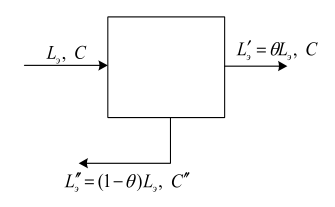
\includegraphics[scale=0.9]{img/sep_el.png}}
  \caption{Схема разделительной ступени }\label{1_1}
\end{figure}


\subsection{Понятие разделительной ступени}


В разделительную ступень параллельно соединяют элементы с одинаковыми величинами $\theta $, $c,$ $ $$c'$ и $c''$ (рис. \ref{1_1}). Она имеет суммарную производительность $L$ и выходящие потоки $L'_{} =\theta L_{}$ и $L''_{} =(1-\theta )L_{}$. Такое представление о работе элементов в ступени предполагает, что все они работают в одинаковых условиях и имеют одинаковые характеристики.

Между приращением $\delta '=c'-c$ и уменьшением $\delta ''=c-c''$ концентрации целевого компонента в выходящих потоках разделительного элемента существует определенная связь. Для стационарного состояния эта связь может быть найдена из следующих уравнений материального баланса:

\begin{equation} \label{GrindEQ__1_1_} 
L=L'+L'', 
\end{equation} 

\begin{equation} \label{GrindEQ__1_2_} 
Lc=L'(c+\delta ')+L''(c-\delta ''). 
\end{equation} 

Из \ref{GrindEQ__1_1_} и \ref{GrindEQ__1_2_} следует, что 

\begin{equation} \label{GrindEQ__1_3_} 
\delta ''=\frac{L'}{L''} \delta '=\frac{\theta }{1-\theta } \delta '. 
\end{equation} 

Одной из основных разделительных характеристик ступени является \textit{полный коэффициент разделения}, который для большинства однофазных методов разделения не зависит от состава изотопной смеси
\begin{equation} \label{GrindEQ__1_4_} 
q={\frac{c'}{1-c'}  \mathord{\left/{\vphantom{\frac{c'}{1-c'}  \frac{c''}{1-c''} =\frac{R'}{R''} }}\right.\kern-\nulldelimiterspace} \frac{c''}{1-c''} =\frac{R'}{R''} } .                              
\end{equation} 

Здесь $R'$ и $R''$ - значения относительной концентрации ценного (целевого) изотопа ($R=\frac{c}{1-c} $) в потоках обогащенной и обедненной фракции. Коэффициент разделения $q$ характеризует эффект разделения, достигаемый в одном элементе или ступени, и может зависеть от производительности ступени $L$ и коэффициента деления потока $\theta $:

\begin{equation} \label{GrindEQ__1_5_} 
q=q(L,\theta ), 
\end{equation} 

где $q(L,\theta )$ - некоторая функция, которую определяют по результатам теоретических или экспериментальных исследований.

В соответствии со сказанным к числу основных параметров ступени относятся восемь величин: $L,\; L',\; L'',\; c,\; c',\; c'',\; q,\; \theta $, связанных независимыми соотношениями \ref{GrindEQ__1_1_}~--\ref{GrindEQ__1_5_}. Причём из перечисленных параметров свободными (независимыми) являются только три. Как правило, в качестве свободных параметров рассматривают величины $L,\; \; c\; $ и $\theta $. Однако, в зависимости от рассматриваемой задачи могут быть выбраны их различные комбинации.

Для удобства анализа эффекта разделения в элементе (ступени) могут быть введены дополнительные параметры и характеристики. Например, коэффициенты разделения по обогащённой $\alpha $ и обеднённой $\beta $ фракциям, рассчитываемые как

\begin{equation} \label{GrindEQ__1_6_} 
\alpha ={\frac{c'}{1-c'}  \mathord{\left/{\vphantom{\frac{c'}{1-c'}  \frac{c}{1-c} }}\right.\kern-\nulldelimiterspace} \frac{c}{1-c} }  , \beta ={\frac{c}{1-c}  \mathord{\left/{\vphantom{\frac{c}{1-c}  \frac{c''}{1-c''} }}\right.\kern-\nulldelimiterspace} \frac{c''}{1-c''} } .        
\end{equation} 

Эти параметры характеризуют величину эффекта разделения в обогащённой и обеднённой фракции по отношению к концентрации в потоке питания. Кроме того, для описания процесса разделения удобно пользоваться коэффициентами обогащения $\varepsilon $, $\varepsilon '$, $\varepsilon ''$, равными

\begin{equation} \label{GrindEQ__1_7_} 
\varepsilon =q-1, \varepsilon '=\alpha -1, \varepsilon ''=1-{1 \mathord{\left/{\vphantom{1 \beta }}\right.\kern-\nulldelimiterspace} \beta } .             
\end{equation} 

Набор параметров $\varepsilon $, $\varepsilon '$, $\varepsilon ''$ позволяет определить \textit{полное обогащение ступени}
\begin{equation} \label{GrindEQ__1_8_} 
\delta =c'-c''=\delta '+\delta '',                          
\end{equation} 

где $\delta '=c'-c$, $\delta ''=c-c''$. Если выразить $c'$ и $c''$ из \ref{GrindEQ__1_6_} и использовать \ref{GrindEQ__1_7_}, то в результате получим
\begin{equation} \label{GrindEQ__1_9_} 
\delta '=\frac{\varepsilon 'c(1-c)}{1+\varepsilon 'c}  ,  \delta ''=\frac{\varepsilon ''c(1-c)}{1-\varepsilon ''c} .              
\end{equation} 

Отсюда видно, что при заданных коэффициентах $\varepsilon '$, $\varepsilon ''$ зависимости $\delta '$ и $\delta ''$ от $c$ имеют максимумы, не совпадающие друг с другом. В случае «слабого обогащения» ($\varepsilon =q-1<<1$) наибольшие значения $\delta '$ и $\delta ''$ достигаются в одной точке $c=0,5$, а формулы \ref{GrindEQ__1_9_} существенно упрощаются:

\begin{equation} \label{GrindEQ__1_10_} 
\delta '=\varepsilon 'c(1-c),  \delta ''=\varepsilon ''c(1-c).              
\end{equation} 

При подстановке \ref{GrindEQ__1_10_} в \ref{GrindEQ__1_8_} имеем

\begin{equation} \label{GrindEQ__1_11_} 
\delta =\varepsilon c(1-c),  \varepsilon '=\varepsilon (1-\theta ), \varepsilon ''=\theta \varepsilon .    
\end{equation} 

Согласно \ref{GrindEQ__1_3_} и \ref{GrindEQ__1_8_} обогащения $\delta $, $\delta '$, $\delta ''$ связаны друг с другом балансовыми соотношениями

\begin{equation} \label{GrindEQ__1_12_} 
\delta '=(1-\theta )\delta ,  \delta ''=\theta \delta .                             
\end{equation} 

Следовательно, если коэффициенты разделения не зависят от параметров $L$ и $\theta $, можно путем уменьшения $\theta $ повысить концентрацию ценного компонента в обогащённом потоке $c'$, произведя таким образом «перераспределение» полного обогащения $\delta $ в выходных потоках. При этом концентрация в обеднённом потоке $c''$ будет приближаться к концентрации во входном потоке $A$. Очевидно, что возможность такого изменения обогащений $\delta '$ и $\delta ''$ связана с условиями сохранения материального баланса в разделительном элементе.

\subsection{Понятие каскада.}


Для получения требуемых концентраций ценного (целевого) изотопа ступени соединяют в последовательную цепочку -- каскад, умножающий эффект разделения в одиночной разделительной ступени. Простейшей схемой последовательного соединения ступеней является так называемый \textit{простой каскад} (рис. \cite{cas}). Его отличительным признаком является подача обогащенной фракции на питание следующей ступени и выведение потоков обедненной фракции ступеней из процесса дальнейшей переработки. В такой схеме поток питания каскада \textit{F} (от английского слова Feed) подают в первую ступень, поток отбора \textit{P} (Product) является потоком обогащенной фракции последней n-ой ступени. Отвальный поток каскада \textit{W} (Waste) образуют обедненные потоки ступеней (могут не смешиваться друг с другом). Так как эти потоки не участвуют в процессе обогащения, то простой каскад, по существу, является прямоточным. Для разделения изотопов, когда разделяемое вещество, как правило, является дорогим, простой каскад является неэффективным. Это обусловлено существенным сокращением потоков питания ступеней и выведением в отвал потоков с концентрацией ценного (целевого) изотопа, близкой к концентрации в обогащенных фракциях. Поэтому при разделении изотопов применяют более эффективную с точки зрения экономии сырья, а также  имеющую ряд других преимуществ, противоточную (рециркуляционную) схему, в которой обедненная ценным компонентом фракция возвращается в каскад для дальнейшей переработки. Простейшая схема такого каскада приведена на рис. \cite{image2}. В этой схеме обогащенный поток $L'_{s} =\theta _{s} L_{s} $ из произвольной $s$-ой ступени подается на вход последующей $s+1$-ой ступени, а обедненный $L''_{s} =(1-\theta _{s} )L_{s} $-- на вход $s-1$-ой ступени. При таком соединении на входе в $s$-ую ступень смешиваются потоки из предыдущей $s-1$-ой ступени и из последующей $s+1$-ой. Такой каскад является \textit{противоточным}, а способ соединения ступеней с помощью внешних коммуникаций, т.е. таких коммуникаций, в которых передаются уже разделенные потоки, называют\textit{ внешним каскадированием}.

\begin{figure}[ht]
  \centerfloat{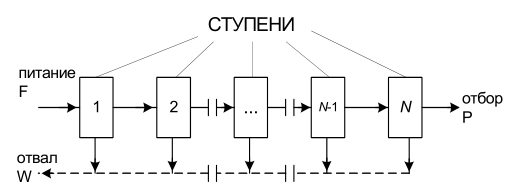
\includegraphics[scale=0.9]{img/cas.png}}
  \caption{Схема простого каскада.}\label{cas}
\end{figure}

\begin{figure}[ht]
  \centerfloat{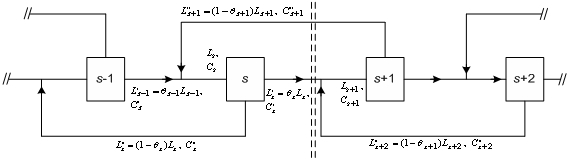
\includegraphics[scale=0.9]{img/image2.png}}
  \caption{Схема соединения ступеней в симметричном противоточном каскаде.}\label{image2}
\end{figure}

Изображенная на рис. \cite{image2}. схема характерна тем, что между любыми соседними ступенями можно провести поперечное сечение (на рисунке изображено двойной пунктирной линией), пересекающее только две коммуникации. Такой каскад называют \textit{симметричным.}

Если потоки направляют не в соседние предыдущую и последующую ступени, а через одну или через несколько ступеней, то такой противоточный каскад называется \textit{несимметричным} (рис. \cite{unsymmetr}).

\begin{figure}[ht]
  \centerfloat{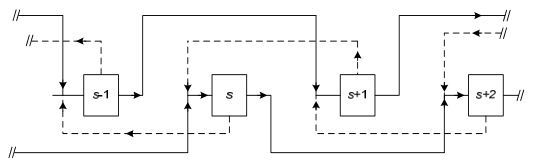
\includegraphics[scale=0.9]{img/unsymmetr.png}}
  \caption{Схема соединения ступеней в несимметричный каскад с подачей потока питания через одну ступень в прямом направлении.}\label{unsymmetr}
\end{figure}


Отметим, что при внешнем каскадировании разделительная ступень считается заданной ячейкой схемы, для которой коэффициент разделения и его зависимость от коэффициента деления потоков должны быть известны, после чего сам процесс разделения оказывается для построения каскадов несущественным. Тем самым теория построения "внешних" потоков оказывается независимой от конкретного метода разделения.

\section{Разделительная способность (мощность). Работа  разделения. Разделительный потенциал.}

В технологии разделения изотопов понятие работы разделения, разделительной мощности и разделительного потенциала имеют весьма важное значение, так как их использование позволяет не прибегая к сложным расчетам оценить необходимое число элементов в каскаде и удельные затраты на производство обогащенного продукта. Количественное определение работы разделения впервые было предложено английскими физиками Пайерлсом и Дираком. Они предположили, что должна существовать функция $\tilde{U}$, с помощью которой можно охарактеризовать «ценность» изотопной смеси как в качественном, так и в количественном отношении, и которую можно представить в виде произведения экстенсивной величины -- количества разделяемой смеси \textit{M} -- на интенсивную величину -- функцию \textit{V(c)}, зависящую только от концентрации ценного изотопа и характеризующую качество смеси

\begin{equation} \label{GrindEQ__1_13_} 
\tilde{U}=MV(C).       
\end{equation} 

Функцию \textit{V(C)}, было предложено называть \textit{разделительным потенциалом}. Необходимо иметь в виду, что функция $\tilde{U}$ ничего общего со стоимостным выражением не имеет и поэтому ее не следует смешивать с реальной ценой изотопной смеси.

Процесс разделения смеси в разделительной установке (Под разделительной установкой здесь будем понимать разделительный каскад, отдельной ячейкой которого является разделительный элемент) для любого метода разделения схематически можно представить следующим образом. До начала процесса имелось некоторое количество исходной смеси \textit{F$^{*}$}(в ед. массы) с концентрацией ценного изотопа \textit{C${}_{F}$}. С использованием введенных понятий изотопная ценность этого смеси будет определяться значением функции $\tilde{U}_{F^{*} } =F^{*} V(С_{F} )$. В результате процесса разделения получают обогащенный продукт в количестве \textit{P${}^{*}$}(в ед. массы) с концентрацией ценного изотопа \textit{C${}_{P}$} и обедненный продукт в количестве \textit{W${}^{*}$}(в ед. массы) с концентрацией \textit{C${}_{W}$}. Изотопная ценность этих продуктов будет $\tilde{U}_{P^{*} } =P^{*} V(C_{P} )$ и $\tilde{U}_{W^{*} } =W^{*} V(C_{W} )$ соответственно. В результате проведения процесса разделения функция $\tilde{U}_{F^{*} } $ изменится на величину $\Delta \tilde{U}$:

\begin{equation} \label{GrindEQ__1_14_} 
\begin{array}{l} {\Delta \tilde{U}=\tilde{U}_{P^{*} } +\tilde{U}_{W^{*} } -\tilde{U}_{F^{*} } =} \\ {=P^{*} V(C_{P} )+W^{*} V(C_{W} )-F^{*} V(C_{F} )} \end{array}           
\end{equation} 

Следовательно «ценность» смеси будет выражаться соотношением

\begin{equation}\label{GrindEQ__1_15_} 
F^{*} V(C_{F} )+\Delta \tilde{U}=P^{*} V(C_{P} )+W^{*} V(C_{W} ).      
\end{equation} 

Из соотношения \ref{GrindEQ__1_15_} следует, что величина $\Delta \tilde{U}$ характеризует меру усилий, которую необходимо затратить на получение из первоначальной бинарной смеси изотопов два новых продукта -- обогащенный и обедненный одним из изотопов этой смеси. Приращение функции $\tilde{U}$, характеризующее перераспределение первоначальной массы разделяемого вещества между двумя выходными потоками и изменение изотопного состава в них при прохождении смеси через разделительную установку, называется \textit{работой разделения}. Введенное понятие работы разделения не имеет ничего общего с реальными энергетическими затратами на поддержание внешних и внутренних потоков в разделительной установке. Из формулы \ref{GrindEQ__1_14_} следует, что введенная таким образом работа разделения имеет размерность количества вещества. 

 Отметим также, что величина работы разделения не дает ответ на вопрос о том, за какое время эта работа может быть выполнена на той или иной разделительной установке. Для получения ответа на это вопрос необходимо знать \textit{разделительную мощность (способность)} установки $\Delta U$, то есть работу разделения, выполняемую установкой в единицу времени. Для перехода от $\Delta \tilde{U}$ к $\Delta U$ достаточно в соотношении \ref{GrindEQ__1_14_} вместо $F^{*} ,P^{*} ,W^{*} $ подставить величины входящего (\textit{F}) и выходящих (\textit{P} и \textit{W}) в установку потоков соответственно.

\begin{equation} \label{GrindEQ__1_16_} 
\Delta U=PV(C_{P} )+WV(C_{W} )-FV(C_{F} ).     
\end{equation} 

Для вычисления работы разделения и разделительной способности необходимо знать явный вид функции \textit{V(C)}. Пайерлс и Дирак решили этот вопрос, рассматривая разделительную способность ступени (элемента), которую в соответствии с вышесказанным можно выразить следующим образом:

\begin{equation} \label{GrindEQ__1_17_} 
\delta U=\theta LV(C')+(1-\theta )LV(C'')-LV(C).   
\end{equation} 

В случае слабого разделения (\textit{q}$\mathrm{\sim}$1) функции $V(A')$ и $V(A'')$ можно разложить в ряд Тейлора в окрестности точки $A$, ограничиваясь членами второго порядка малости

\begin{equation} \label{GrindEQ__1_18_} 
V(A')\approx V(A)+\frac{dV}{dA} \delta '+\frac{1}{2} \frac{d^{2} V}{dA^{2}} (\delta ')^{2} ,        
\end{equation}

\begin{equation} \label{GrindEQ__1_19_} 
V(A'')\approx V(A)-\frac{dV}{dA} \delta ''+\frac{1}{2} \frac{d^{2} V}{dA^{2} } (\delta '')^{2} .     
\end{equation} 

Подставив их в \ref{GrindEQ__1_17_}, находим

\begin{equation} \label{GrindEQ__1_20_} 
\begin{array}{l} {\delta U=\left[\theta L+(1-\theta )L-L\right]{\kern 1pt} {\kern 1pt} {\kern 1pt} V(A)+\left[\theta L\delta '-(1-\theta )L\delta ''\right]\frac{dV}{dA} +} \\ {\, \, \, \, \, \, \, \, \, \, \, \, \, \, \, \, \, \, \, \, \, +\frac{1}{2} \left[\theta L(\delta ')^{2} +(1-\theta )L(\delta '')^{2} \right]\frac{d^{2} V}{dA^{2} } \, \, \, .} \end{array} 
\end{equation} 

Из условий баланса \ref{GrindEQ__1_1_}, \ref{GrindEQ__1_2_} и \ref{GrindEQ__1_12_} коэффициенты при $V(A)$ и ${dV \mathord{\left/{\vphantom{dV dA}}\right.\kern-\nulldelimiterspace} dA} $ равны нулю. Поэтому с учётом \ref{GrindEQ__1_11_} и \ref{GrindEQ__1_12_} имеем

\begin{equation} \label{GrindEQ__1_21_} 
\delta U=\frac{1}{2} \theta (1-\theta )L\varepsilon ^{2} \frac{d^{2} V}{dA^{2} } A^{2} (1-A)^{2} .           
\end{equation} 

Пайерлс и Дирак ввели условие, согласно которому разделительная способность (мощность) ступени или элемента определяется только его разделительными характеристиками $L,\; \theta ,\; \varepsilon $ и не должна зависеть от состава питающей его смеси. Это условие обосновывается следующим соображением. Если разделительная способность отдельной ячейки установки -- разделительного элемента -- не зависит от концентрации и все элементы работают в идентичных условиях, то есть с одинаковыми $L,\; \theta ,\; \varepsilon $, то суммарная разделительная способность элементов, составляющих эту установку, будет равна произведению $Z\cdot \delta U_{M;} $, где $\delta U_{M;} $ - разделительная способность одного элемента, \textit{Z} --число элементов в установке. Если процесс разделения организован так, что потери работы разделения (разделительной способности) отсутствуют, то величина $Z\cdot \delta U_{M;} $ будет равна разделительной способности всей установки $\Delta U$, вычисляемой по формуле \ref{GrindEQ__1_16_}, то есть

\begin{equation} \label{GrindEQ__1_22_} 
\Delta U=Z\cdot \delta U_{M;} .       
\end{equation} 

Откуда число разделительных элементов в каскаде будет определяться по формуле

\begin{equation} \label{GrindEQ__1_23_} 
Z=\frac{\Delta U}{\delta U_{M;} }  .        
\end{equation} 

Таким образом, если условие независимости разделительной способности от концентрации выполнено, то появляется возможность вычислить важную характеристику процесса разделения -- суммарное число элементов, обеспечивающих необходимую разделительную способность установки для решения заданной разделительной задачи.

Условие независимости разделительной способности ступени (элемента) от концентрации приводит к следующему уравнению:

\begin{equation} \label{GrindEQ__1_24_} 
\delta U=\frac{1}{2} \theta (1-\theta )L\varepsilon ^{2} \frac{d^{2} V}{dc^{2} } c^{2} (1-c)^{2} =const.   
\end{equation} 

Если в уравнении \ref{GrindEQ__1_24_} выбрать постоянную в виде

\begin{equation} \label{GrindEQ__1_25_} 
const=\frac{1}{2} \theta (1-\theta )L\varepsilon ^{2} ,     
\end{equation}

то для определения потенциала \textit{V}(\textit{c}) получается дифференциальное уравнение

\begin{equation} \label{GrindEQ__1_26_} 
\frac{d^{2} V}{dc^{2} } =\frac{1}{c^{2} (1-c^{2} )} ,      
\end{equation}

общее решение которого имеет вид:

\begin{equation} \label{GrindEQ__1_27_} 
V(c)=(2c-1)\ln \frac{c}{1-c} +ac+b.    
\end{equation} 

Произвольные постоянные в выражении \ref{GrindEQ__1_27_} должны быть определены дополнительными условиями. Однако нетрудно видеть, что эти постоянные не имеют существенного значения, так как при вычислении работы разделения по формуле \ref{GrindEQ__1_15_} или разделительной способности по формуле \ref{GrindEQ__1_16_} они не входят в окончательный результат с учетом уравнений материального баланса. Поэтому, следуя Пайерлсу, можно положить $a=b=0$ и тогда потенциал приобретает вид

\begin{equation} \label{GrindEQ__1_28_} 
V(C)=(2A-1)\ln \frac{A}{1-A}.                            
\end{equation} 

\begin{figure}[ht]
  \centerfloat{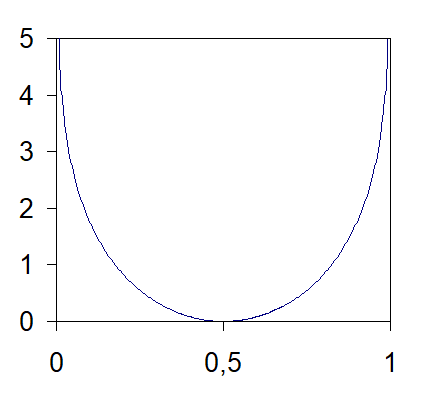
\includegraphics[scale=0.6]{img/image1}}
  \caption{Зависимость разделительного потенциала от концентрации.}\label{image1}
\end{figure}

В этой форме его обычно называют потенциалом Пайерлса-Дирака. Графический вид функции $V(A)$ показан на рис. \ref{image1}. 

Разделительный потенциал Пайерлса-Дирака и его производная равны нулю при \textit{с}=0,5. При любых других значениях концентрации потенциал \textit{V}(\textit{c})$\mathrm{>}$0, а при \textit{с}$\rightarrow$0 или \textit{с}$\rightarrow$$\propto$ потенциал \textit{V}(\textit{c}) $\rightarrow$$\propto$, что означает необходимость бесконечно большой работы разделения для получения чистых изотопных продуктов.

Таким образом, в случае «слабого обогащения» разделительный потенциал определяется формулой \ref{GrindEQ__1_28_}, а разделительная способность -- соотношением \ref{GrindEQ__1_25_}.

Какой физический смысл имеет разделительная способность? Пайерлс и Фукс установили прямую связь величины $\delta U$ с уменьшением энтропии смеси в единицу времени $\Delta S_\textup{разд.}$, которое имеет место при стационарной работе разделительной ступени (элемента). Величину $\Delta S_\textup{разд.}$ можно рассчитать из следующих соображений. Энтропия при образовании одного моля смеси идеальных газов или сильно разбавленного раствора из чистых компонентов равна 

\begin{equation} \label{GrindEQ__1_29_} 
S=-\tilde{R}\left[c\ln c+(1-c)\ln (1-c)\right],       
\end{equation} 

где $\tilde{R}$ - газовая постоянная.

Если из \textit{L} молей питающей смеси с концентрацией \textit{C} получается на выходе ступени (элемента) в единицу времени $L'=\theta L$ молей обогащенного до концентрации $C'$, и $L''=(1-\theta )L$ молей, обедненных до концентрации $C''$, то изменение энтропии в единицу времени $\Delta S_\textup{разд.}$ будет равно

\begin{equation} \label{GrindEQ__1_30_} 
\Delta S_\textup{разд.} =\mathrm{\; -}\left[LS(C)-\theta LS(C')-(1-\theta )LS(C'')\right].    
\end{equation} 

В случае «слабого разделения» выражение для $\Delta S_\textup{разд.} $ заметно упрощается, если соотношение \ref{GrindEQ__1_30_} представить в виде

\begin{equation} \label{GrindEQ__1_31_} 
\Delta S_\textup{разд.} =\theta LS(C+\delta ')+(1-\theta )LS(C-\delta '')-LS(C).   
\end{equation} 

Разлагая в ряд функции $S(C+\delta ')$ и $S(C-\delta '')$ в ряд Тейлора в окрестности точки \textit{C} и ограничиваясь членами второго порядка малости, после несложных преобразований получаем

\begin{equation} \label{GrindEQ__1_32_} 
\Delta S_\textup{разд.} =\frac{\theta (1-\theta )}{2} \delta ^{2} \frac{d^{2} S}{dc^{2} } .       
\end{equation} 

Учитывая, что $\delta =\varepsilon c(1-c)$ и $\frac{d^{2} S}{dc^{2} } =-\frac{\tilde{R}}{c(1-c)} $, и подставляя выражение \ref{GrindEQ__1_32_} в \ref{GrindEQ__1_31_}, получим

\begin{equation} \label{GrindEQ__1_33_} 
\Delta S_\textup{разд.} =-\frac{\theta (1-\theta )}{2} L\varepsilon ^{2} \tilde{R}C(1-C),      
\end{equation} 

которое с учетом выражения \ref{GrindEQ__1_25_} может быть переписано в виде

\begin{equation} \label{GrindEQ__1_34_} 
\Delta S_\textup{разд.} =-\delta U\cdot \tilde{R}C(1-C)       
\end{equation} 

Из полученного выражения \ref{GrindEQ__1_34_} следует, что величина разделительной способности $\delta U$ прямо пропорциональна уменьшению величины безразмерной энтропии смеси $\Delta S_\textup{разд.} /\tilde{R}$. Изменение концентраций компонентов в смеси газов связано с изменением меры порядка. В общем случае мерой порядка служит энтропия. В соответствии с \ref{GrindEQ__1_34_} уменьшение энтропии при разделении на ступени произведению концентраций компонентов изотопной смеси \textit{c}(1-\textit{c}). Это произведение определяет вероятность нахождения в смеси пары различных молекул. Вследствие этого разделительная способность ступени равна уменьшению безразмерной энтропии, отнесенной к величине этой вероятности. Таким образом, разделительная ступень увеличивает меру порядка в смеси изотопов. Скорость увеличения этой меры определяет разделительную способность ступени. 

Перейдем теперь к случаю, когда коэффициент разделения ступени \textit{q} заметно отличается от единицы. При произвольных значениях полного коэффициента разделения \textit{q} функциональное уравнение 
\begin{equation} \label{GrindEQ__1_35_} 
\delta U=\theta LV(C')+(1-\theta )LV(C'')-LV(C)=const 
\end{equation} 

имеет решение, при котором функция \textit{V} зависит только от концентрации в случае симметричной работы ступени, то есть когда $\alpha =\beta =\sqrt{q} $ [1].

 Если процесс разделения в ступени симметричен, то выполняются условия

 \begin{equation} \label{GrindEQ__1_36_} 
R'=\alpha R,\; \; R''=\frac{1}{\alpha } R,\; \; \theta =\frac{1+\alpha R}{(\alpha +1)(1+R)} ,\; \; 1-\theta =\frac{\alpha +R}{(\alpha +1)(1+R)} , 
\end{equation} 
где $R=\frac{C}{1-C} $.

 Подставляя \ref{GrindEQ__1_36_} в \ref{GrindEQ__1_35_}, имеем 
\begin{equation} \label{GrindEQ__1_37_} 
\frac{\delta U}{L} =\frac{1+\alpha R}{(\alpha +1)(1+R)} V(\alpha R)+\frac{\alpha (1+\frac{R}{\alpha } )}{(\alpha +1)(1+R)} V\left(\frac{R}{\alpha } \right)-V(R)=const. 
\end{equation} 

Введем новую переменную \textit{l} следующим образом:
\begin{equation} \label{GrindEQ__1_38_} 
R=R_{0} \alpha ^{l} ,       
\end{equation} 

где \textit{R}${}_{0}$ -- константа, и положим, что
\begin{equation} \label{GrindEQ__1_39_} 
(1+R)V(R)\equiv F(l).     
\end{equation} 

С учетом \ref{GrindEQ__1_38_} и \ref{GrindEQ__1_39_} уравнение \ref{GrindEQ__1_37_} трансформируется в классическое разностное уравнение второго порядка
\begin{equation} \label{GrindEQ__1_40_} 
F(l+1)+\alpha F(l-1)-(\alpha +1)F(l)=A(\alpha +1)(1+R_{0} \alpha ^{l} ),   
\end{equation} 

где \textit{A} -- константа.

Общее решение уравнения \ref{GrindEQ__1_40_} можно представить в виде
\begin{equation} \label{GrindEQ__1_41_} 
F(l)=A\frac{\alpha +1}{\alpha -1} l(R_{0} \alpha ^{l} -1)+a\alpha ^{l} +b),    
\end{equation} 

где \textit{a }и \textit{b} также константы.

Используя выражения \ref{GrindEQ__1_37_} и \ref{GrindEQ__1_41_}, найдем вид функции \textit{V}(\textit{R)}
\begin{equation} \label{GrindEQ__1_42_} 
V(R)=A\frac{\alpha +1}{(\alpha -1)\ln \alpha } \left[(2c-1)\ln \frac{R}{R_{0} } +a\ln \alpha \frac{c}{R} +b\ln \alpha (1-c)\right].  
\end{equation} 

Выбирая константу \textit{A} равной $A=\frac{\delta U}{L} =\frac{\alpha -1}{\alpha +1} \ln \alpha $ и полагая, что $R_{0} =1,\quad a=0,\quad b=0$${}^{*}$ (Как и в случае «слабого обогащения», эти константы не входят в окончательные выражения для разделительного потенциала и разделительной способности), получим для разделительного потенциала и разделительной способности следующие выражения:

\begin{equation} \label{GrindEQ__1_43_} 
V(c)=(2c-1)\ln \frac{c}{1-c} ,        
\end{equation} 

\begin{equation} \label{GrindEQ__1_44_} 
\delta U=L\frac{(\alpha -1)\ln \alpha }{\alpha +1} \equiv L\frac{\left(\sqrt{q} -1\right)\ln \sqrt{q} }{\sqrt{q-1} } .     
\end{equation} 

Очевидно, что в случае «слабого разделения» $(\varepsilon =q-1<<1)$ формула \ref{GrindEQ__1_44_} переходит в формулу \ref{GrindEQ__1_25_} при $\theta =1/2$. Отметим, что соотношения \ref{GrindEQ__1_25_}, \ref{GrindEQ__1_28_} и \ref{GrindEQ__1_44_}, полученные на основе подхода Пайерлса-Дирака, полностью подтверждаются результатами теории идеальных каскадов из симметричных ступеней, разработанной К.Коэном.

В случае несимметричной работы ступени $(\alpha \ne \beta )$ при произвольном обогащении на ступени выполнить оба условия Пайерлса-Дирака, а именно

- разделительный потенциал зависит только от изотопного состава смеси;

- разделительная способность ступени определяется только характеристиками самой ступени;

не удается. Разделительная способность ступени зависит от коэффициентов разделения $(\alpha ,\beta)$ и концентрации смеси. Как будет показано ниже, при больших $(1-c<<1)$ и малых $(c<<1)$ концентрациях величина $\delta U$ от концентрации не зависит. Разделительный потенциал, полученный из решения функционального уравнения \ref{GrindEQ__1_35_} оказывается зависящим не только от состава смеси, но и коэффициентов разделения ступени, то есть $V(c,\alpha ,\beta)$.

На основе разделительного потенциала, записанного в виде \ref{GrindEQ__1_28_}, введены единицы работы разделения изотопов урана. В настоящее время его используют и в случае произвольных коэффициентов разделения на ступени, работающей в несимметричном режиме [38, 52]. Теоретическое обоснование подобного подхода, проведенного в различных работах, связано, в частности, с изменением условий Пайерлса-Дирака \cite{baranovIzotopySvoystvaPoluchenie} и рассмотрением идеализированного процесса разделения \cite{yamamotoMulticomponentIsotopeSeparating1978}.

Исходя из общего соотношения для разделительной способности ступени
\begin{equation} \label{GrindEQ__1_45_} 
\delta U=\theta LV(c')+(1-\theta )LV(c'')-LV(c) 
\end{equation} 

и разделительного потенциала, определяемого по формуле \ref{GrindEQ__1_28_}, можно найти формулу при всех значениях $q$ и $(\alpha \ne \beta )$ [8, 9]. Поскольку $A=\frac{R}{R+1} ,\; \; 2A-1=\frac{R-1}{R+1} $, разделительный потенциал \ref{GrindEQ__1_28_} может быть представлен в виде

\begin{equation} \label{GrindEQ__1_46_} 
V^{*} (R)=\frac{R-1}{R+1} \ln R,                            
\end{equation} 

где индекс «звездочка» означает то, что разделительный потенциал рассматривается как функция новой переменной $R$.

Соотношение для определения разделительной способности ступени запишется в виде

\begin{equation} \label{GrindEQ__1_47_} 
\delta U=L[\theta V^{*} (R')+(1-\theta )V^{*} (R'')-V(R)].    
\end{equation} 

Формулу для определения коэффициента деления потока нетрудно получить, комбинируя выражения \ref{GrindEQ__1_3_}, \ref{GrindEQ__1_7_} и \ref{GrindEQ__1_9_}:

\begin{equation} \label{GrindEQ__1_48_} 
\theta =\frac{\left(\beta -1\right)\left[1+(\alpha -1)c\right]}{\alpha \beta -1} .        
\end{equation} 

Замена в \ref{GrindEQ__1_48_} концентрации \textit{с} на отношение $R/(1-R)$ приводит к выражениям

\begin{equation} \label{GrindEQ__1_49_} 
\theta =\frac{\left(\alpha R+1\right)\mathrm{\; }\left(\beta -1\right)}{\left(R+1\right)\mathrm{\; }\left(\alpha \beta -1\right)} ,         
\end{equation} 
\begin{equation} \label{GrindEQ__1_50_} 
1-\theta =\frac{\left(R+\beta \right)\mathrm{\; }\left(\alpha -1\right)}{\left(R+1\right)\mathrm{\; }\left(\alpha \beta -1\right)} .         
\end{equation} 

Подставляя \ref{GrindEQ__1_46_}, \ref{GrindEQ__1_49_} и \ref{GrindEQ__1_50_} в \ref{GrindEQ__1_47_} с учетом $R'=\alpha R,\; R''=\frac{1}{\beta } R$ и $\alpha \beta =q$, получим

\begin{equation} \label{GrindEQ__1_51_} 
\begin{array}{l} {\delta U=L\frac{1}{q-1} \left\{\left[\left(\alpha -1\right)\beta \ln \beta -\left(\beta -1\right)\ln \alpha \right]\frac{1}{R+1} +\right. } \\ {\left. +\left[\left(\beta -1\right)\alpha \ln \alpha -\left(\alpha -1\right)\ln \beta \right]\frac{R}{R+1} \right\}} \end{array}.  
\end{equation} 

Переходя в \ref{GrindEQ__1_51_} от относительных концентраций \textit{R} к абсолютным, окончательно получим

\begin{equation} \label{GrindEQ__1_52_} 
\delta U=L[f_{1} (\alpha ,\beta )(1-A)+f_{2} (\alpha ,\beta )A], 
\end{equation} 

где
\begin{equation} \label{GrindEQ__1_53_} 
  f_{1} (\alpha ,\beta )=\frac{(\alpha -1)\beta \ln \beta -(\beta -1)\ln \alpha }{\alpha \beta -1} ,  
\end{equation} 

\begin{equation} \label{GrindEQ__1_54_} 
f_{2} (\alpha ,\beta )=\frac{(\beta -1)\alpha \ln \alpha -(\alpha -1)\ln \beta }{\alpha \beta -1} ,  
\end{equation} 

Из \ref{GrindEQ__1_52_} следует, что разделительная способность ступени $\delta U$ в общем случае является функцией концентрации. Зависимость от концентрации исчезает в следующих частных случаях.

1. Случай слабого разделения, $\alpha -1<<1,\; \; \beta -1<<1$. Так как в этом случае $\alpha $~и~$\beta $ близки к единице, то

\begin{equation} \label{GrindEQ__1_55_} 
\ln \alpha \approx (\alpha -1)-\frac{1}{2} (\alpha -1)^{2} +\cdot \cdot \cdot , 
\end{equation} 

\begin{equation} \label{GrindEQ__1_56_} 
\ln \beta \approx (\beta -1)-\frac{1}{2} (\beta -1)^{2} +\cdot \cdot \cdot , 
\end{equation} 

Имея в виду \ref{GrindEQ__1_7_}, \ref{GrindEQ__1_11_} и \ref{GrindEQ__1_12_}, подставляя \ref{GrindEQ__1_55_} и \ref{GrindEQ__1_56_} в \ref{GrindEQ__1_52_} и сохраняя малые величины 2-ого порядка, имеем
\begin{equation} \label{GrindEQ__1_57_} 
\delta U=\frac{L}{2} (\alpha -1)(\beta -1)\approx \frac{L}{2} \varepsilon '\varepsilon ''=\frac{\theta (1-\theta )L\varepsilon ^{2} }{2} ,             
\end{equation} 

что соответствует классическому виду для разделительной способности \ref{GrindEQ__1_25_}.

2. Случай симметричной ступени при произвольном на ней обогащении. При $\alpha =\beta $ \ref{GrindEQ__1_52_} преобразуется к виду
\begin{equation} \label{GrindEQ__1_58_} 
\delta U=L\frac{(\alpha -1)\alpha \ln \alpha -(\alpha -1)\ln \alpha }{\alpha ^{2} -1} =L\frac{(\alpha -1)\ln \alpha }{\alpha +1} ,              
\end{equation} 

что также соответствует классической формуле \ref{GrindEQ__1_44_}.

3. Случай малых концентраций, $A<<1.$ При $A<<1,\; \; 1-A\approx 1$ выражение \ref{GrindEQ__1_52_} преобразуется к виду
\begin{equation} \label{GrindEQ__1_59_} 
\delta U=Lf_{1} (\alpha ,\beta )=L\frac{(\alpha -1)\beta \ln \beta -(\beta -1)\ln \alpha }{\alpha \beta -1} .                     
\end{equation} 

В рассматриваемом случае выражение \ref{GrindEQ__1_49_} упрощается
\begin{equation} \label{GrindEQ__1_60_} 
\theta =\frac{\beta -1}{\alpha \beta -1} .                                        
\end{equation} 

Соответственно, величина $\beta $ равна
\begin{equation} \label{GrindEQ__1_61_} 
\beta =1+\theta (\alpha \beta -1).                            
\end{equation} 

Учёт \ref{GrindEQ__1_60_} и \ref{GrindEQ__1_61_} и связи$\alpha \beta =q$ позволяет преобразовать соотношение \ref{GrindEQ__1_59_} к виду
\begin{equation} \label{GrindEQ__1_62_} 
\delta U=L\{ \ln [1+\theta (q-1)]-\theta \ln q\} .            
\end{equation} 

Это выражение для разделительной способности имеет важное значение при расчетах каскадов для получения слабообогащенного урана. 

4. В случае больших концентраций, когда выполняется $(c\approx 1)$ выражение \ref{GrindEQ__1_42_} преобразуется к виду
\begin{equation} \label{GrindEQ__1_63_} 
\delta U=Lf_{2} (\alpha ,\, \beta )=L\frac{\beta (\alpha -1)\ln \beta -(\beta -1)\ln \alpha }{q-1} .     
\end{equation} 

В этом случае коэффициент деления потока запишется как
\begin{equation} \label{GrindEQ__1_64_} 
\theta =\frac{q(\beta -1)}{\beta (q-1)} ,         
\end{equation} 

а выражение для разделительной способности с учётом соотношения $q=\alpha \beta $ будет иметь вид
\begin{equation} \label{GrindEQ__1_65_} 
\delta U=L\left\{\ln \left[q-\theta (q-1)\right]-(1-\theta )\ln q\right\}.      
\end{equation} 

Коэффициент разделения по обеднённой фракции $\beta $ в формуле для разделительной способности \ref{GrindEQ__1_52_} можно выразить через $\alpha $. Тогда после дифференцирования удельной разделительной способности $\delta U/L$ по $\alpha $ и приравнивания производной нулю, получим квадратное уравнение относительно $\alpha $ [10, 22]:

\begin{equation} \label{GrindEQ__1_66_} 
a\alpha ^{2} -b\alpha -d=0,          
\end{equation} 

в котором $a=c\frac{\ln q}{q-1} ,\quad b=2c-1,\quad d=(1-c)\frac{\ln q}{q-1} \mathrm{\; }q\; .$

Квадратное уравнение \ref{GrindEQ__1_66_} имеет только одно физическое решение, обеспечивающее максимум величины $\delta U/L$:
\begin{equation} \label{GrindEQ__1_67_} 
\alpha_\textup{опт.} =\frac{q}{\beta_\textup{опт.}} =\frac{b+\sqrt{b^{2} +4ad} }{2} .      
\end{equation} 

Нетрудно видеть, что, во-первых, решение \ref{GrindEQ__1_67_} зависит от величин $q$ и $C$, а, во-вторых, независимо от величины $q$ при $C=0,5$ максимальное значение $\alpha_\textup{опт.} $ будет равно $\alpha_\textup{опт.} =\sqrt{q}$. Следовательно, максимум удельной разделительной способности ступени при значении концентрации $C=0,5$ достигается в соответствии \ref{GrindEQ__1_67_} при симметричном режиме работы ступени, то есть при условии $\alpha $=$\beta $. При концентрациях, отличных от 0,5, максимум удельной разделительной способности не соответствует симметричному режиму работы разделительной ступени. Для интересного для практики случая $C<<1$ (получение слабообогащённого урана) отыскание максимума функции приводит к следующим значениям [11]

\begin{equation} \label{GrindEQ__1_68_} 
\theta_\textup{опт.} =\frac{1}{\ln q} -\frac{1}{q-1} ,        
\end{equation} 
\begin{equation} \label{GrindEQ__1_69_} 
\alpha_\textup{опт.} =\frac{q}{\beta_\textup{опт.}} =\frac{q\ln q}{q-1} ,        
\end{equation} 
\begin{equation} \label{GrindEQ__1_70_} 
\left(\frac{\delta U}{L} \right)_{\max } =\ln \left[\frac{(q-1)}{\ln q} \right]+\frac{\ln q}{q-1} -1.    
\end{equation} 

Отметим, что выражение \ref{GrindEQ__1_69_} для $\alpha_\textup{опт.} $ может быть получено из \ref{GrindEQ__1_67_} подстановкой условия $C<<1$.

% В таблице 1.1 приведены величины $\theta ,\; \alpha ,\; \beta \; $ и $\delta U/L$ разделительной ступени для симметричного случая $(\alpha =\beta )$ и случая, когда ступень работает с оптимальной величиной $\theta $ в зависимости от величины \textit{q} при малых концентрациях ценного компонента (\textit{с}$\mathrm{<}$$\mathrm{<}$1).

% Таблица 1.1.

% \noindent Характеристики разделительной ступени каскада при симметричном и оптимальном разделении для различных значений \textit{q} и \textit{с}$\mathrm{<}$$\mathrm{<}$1

% \begin{tabular}{|p{0.7in}|p{0.5in}|p{0.4in}|p{0.4in}|p{0.4in}|p{0.5in}|} \hline 
% \textit{q} & 1,1 & 1,6 & 3,0 & 5,0 & 10,0 \\ \hline 
% \textit{$\theta$}${}_{\textrm{с}\textrm{и}\textrm{м}}$ & 0,488 & 0441 & 0,366 & 0,309 & 0,240 \\ \hline 
% \textit{$\theta$}${}_{\textrm{о}\textrm{п}\textrm{т}}$ & 0,492 & 0,461 & 0,401 & 0,371 & 0,323 \\ \hline 
% \textit{$\alpha$}${}_{\textrm{с}\textrm{и}\textrm{м}}$ & 1,0488 & 1,2649 & 1,7320 & 2,2361 & 3,1623 \\ \hline 
% \textit{$\alpha$}${}_{\textrm{о}\textrm{п}\textrm{т}}$ & 1,0484 & 1,2532 & 1,6780 & 2,0118 & 2,5584 \\ \hline 
% \textit{$\beta$}${}_{\textrm{с}\textrm{и}\textrm{м}}$ & 1,0488 & 1,2649 & 1,7320 & 2,2361 & 3,1623 \\ \hline 
% \textit{$\beta$}${}_{\textrm{о}\textrm{п}\textrm{т}}$ & 1,0492 & 1,2766 & 1,8204 & 2,4853 & 3,9087 \\ \hline 
% $\left(\delta U/L\right)$${}_{\textrm{с}\textrm{и}\textrm{м}}$ & 1,134$.$10${}^{-3}$ & 0,0275 & 0,1471 & 0,3075 & 0,5980 \\ \hline 
% $\left(\delta U/L\right)$${}_{\textrm{м}\textrm{а}\textrm{к}\textrm{с}}$ & 1,135$.$10${}^{-3}$ & 0,0276 & 0,1483 & 0,3128 & 0,6190 \\ \hline 
% $\frac{\left(\delta U/L\right)_{<0:A} -\left(\delta U/L\right)_{A8<} }{\left(\delta U/L\right)_{A8<} } $,\% & 0,088 & 0,364 & 0,817\newline  & 1,723 & 3,512 \\ \hline 
% \end{tabular}

% Видно, что с возрастанием \textit{q} увеличивается разница между максимально возможным значением $\left(\delta U/L\right)$${}_{\textrm{м}\textrm{а}\textrm{к}\textrm{с}}$, получаемым при $\alpha \ne \beta $, и $\left(\delta U/L\right)$${}_{\textrm{с}\textrm{и}\textrm{м}}$, соответствующим симметричному разделению в ступени.

% Как будет показано в разделе 1.8 рассмотренные особенности разделения существенны для анализа эффективности работы многоступенчатых установок.

\section{Получение уравнений симметрично-противоточного каскада для случая произвольного числа компонентов и произвольных коэффициентов разделения.}

Рассмотрим симметричный каскад, состоящий из \textit{N} ступеней. 

Пусть на вход ступени с номером $s=f$ подают поток питания $F$ с концентрацией $A_{F} $. Поток, обогащенный ценным (целевым) изотопом, отбирается с правого конца каскада $(s=N)$ (сокращенно: отбор), а обедненный поток - с левого конца каскада $(s=1)$ (сокращенно: отвал). Соответственно обозначим концентрации в потоках отбора $A_{P} $ и отвала $A_{W} $. Ступени каскада нумеруются последовательно от 1 на отвале до \textit{N} на отборе. Часть каскада от точки подачи питания $(s=f,\; \; f+1,\; { ...}\; {,}\; \; {N)}$ называется обогатительной, а часть слева $(s=1,\; \; 2,\; \; {...}\; {,}\; \; f{ -1)}$ - обеднительной.

В симметричной противоточной схеме можно использовать частичный или полный возврат обогащённых или обеднённых потоков отбора или отвала на вход соответствующей ступени $(s=N$ или $s=1)$. Такие коммутации потоков называют "закрутками" и обычно их применяют на концевых ступенях каскада [5] (рис. \ref{loop}).

\begin{figure}[ht]
  \centerfloat{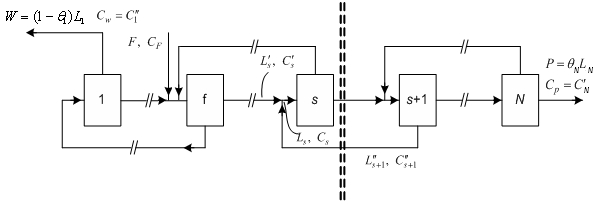
\includegraphics[scale=0.6]{img/image3.png}}
  \caption{Схема симметричного каскада для разделения бинарных смесей.}\label{loop}
\end{figure}

\begin{figure}[ht]
  \centerfloat{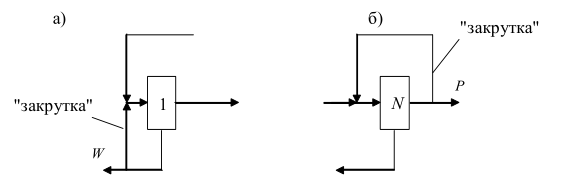
\includegraphics[scale=0.99]{img/loop.png}}
  \caption{Схемы закруток потоков : а) -- на отвале; б) -- на отборе.}\label{loop}
\end{figure}


Внешними параметрами каскада являются шесть переменных, определяющих внешние рабочие условия: $F,\; P,\; W$ - потоки питания, отбора и отвала каскада; $A_{F} ,\; A_{P} ,\; A_{W}$ - концентрации в соответствующих потоках. К внутренним относятся: \textit{N} -- общее количество ступеней в каскаде, \textit{f} -- номер ступени, на вход которой подают поток питания, параметры ступеней: $L_{S} ,\; L'_{S} ,\; L''_{S} $ - входной и два выходных потока на s-ой ступени каскада, $A_{S} ,\; A'_{S} ,\; A''_{S} \; $- концентрации в соответствующих потоках; $q_{S} ,\; \alpha _{S} ,\; \beta _{S} $ - коэффициенты разделения и $\theta _{S} $ - коэффициенты деления потоков $(s=\overline{1,N)}$.

В стационарном состоянии каскада внутренние параметры каскада можно выразить через внешние параметры каскада и уравнения разделения в ступени. Проведем поперечное сечение между некоторой \textit{s} -- ой ступенью и соседней с ней \textit{s}+1 -- ой ступенью обогатительной части каскада (обозначено на рис. \ref*{loop} пунктиром) и рассмотрим часть каскада, находящуюся справа от этого мысленного сечения. Потоки разделяемого вещества и потоки ценного (целевого) изотопа входящие в эту часть каскада $L'_{S} =\theta _{S} L_{S} $ и $L'_{S} A'_{S} =\theta _{S} L_{S} A_{s}^{/} $ и выходящие из нее $L''_{S+1} =(1-\theta _{S+1} )L_{S+1} $ и $L''_{S+1} A''_{S+1} =(1-\theta _{S+1} )L_{S+1} A''_{S+1} $ связаны уравнениями материального баланса:

\begin{equation} \label{GrindEQ__1_71_} 
\theta _{S} L_{S} -(1-\theta _{S+1} )L_{S+1} =P,                
\end{equation} 

\begin{equation} \label{GrindEQ__1_72_} 
\theta _{S} L_{S} C'_{S} -(1-\theta _{S+1} )L_{S+1} C''_{S+1} =PC_{P}.     
\end{equation} 

В этих уравнениях через, $C'_{s}$ и $C''_{s}$ обозначены концентрации ценного (целевого) изотопа соответственно на выходах из ступени.

Аналогичные соотношения можно записать для обеднительной части каскада

\begin{equation} \label{GrindEQ__1_73_} 
  \theta _{s} L_{s} -(1-\theta _{s+1} )L_{s+1} =-W, 
\end{equation}

\begin{equation} \label{GrindEQ__1_74_} 
  \theta _{s} L_{s} c'_{s} -(1-\theta _{s+1})L_{s+1} c''_{s+1} =-WC_{w}. 
\end{equation} 

Для ступени с номером \textit{s=f}, на вход которой подают поток питания \textit{F}, уравнения материального баланса имеют вид
\begin{equation} \label{GrindEQ__1_75_} 
L_{f} =\theta _{f-1} L_{f-1} +(1-\theta _{f+1} )L_{f+1} +F,     
\end{equation}

\begin{equation} \label{GrindEQ__1_76_}
  L_{f} c_{f} = \theta _{f-1} L_{f-1} c'_{f-1} + (1-\theta _{f+1})L_{f+1} c''_{f+1} +Fc_{F}.  
\end{equation}

При использовании формул \ref{GrindEQ__1_71_} -- \ref{GrindEQ__1_74_} следует иметь в виду, что $L_{0} =0$ и $L_{N+1} =0$. Концентрации $c_{S} ,\; c'_{S} $ и $c''_{S} $ на каждой ступени связаны соотношениями \ref{GrindEQ__1_4_}, \ref{GrindEQ__1_6_}, \ref{GrindEQ__1_7_}, а внешние параметры при отсутствии потерь вещества в ступенях каскада должны удовлетворять уравнениям материального баланса:
\begin{equation} \label{GrindEQ__1_77_} 
F=P+W,                                       
\end{equation} 
\begin{equation} \label{GrindEQ__1_78_} 
Fc_{F} {}^{} =Pc_{P} {}^{} +Wc_{W} {}^{} .                      
\end{equation} 

Вводя для разности концентраций на входах двух произвольных соседних  ступеней обозначение

\begin{equation} \label{GrindEQ__1_79_} 
\Delta _{S} =c_{S+1} -c_{S} ,\; (s=1,N-1) 
\end{equation} 

и, вычитая соотношение \ref{GrindEQ__1_71_}, умноженное на $c_{S} $, из \ref{GrindEQ__1_72_}, получим

\begin{equation} \label{GrindEQ__1_80_} 
\Delta _{S} =\frac{\theta _{S} L_{S} }{(1-\theta _{S+1} )L_{S+1} } \delta '_{S} +\delta ''_{S+1} -\frac{P(c_{P} -c_{S} )}{(1-\theta _{S+1} )L_{S+1} } ,            
\end{equation} 

где величины $\delta '_{S} =c'_{S} -c_{S} $ и$\delta ''_{S} =c_{S} -c''_{S} $ определяются соотношениями \ref{GrindEQ__1_9_}, \ref{GrindEQ__1_7_}. Для обеднительной части каскада справедливы точно такие же уравнения, только в правой части вместо \textit{P} и $Pc_{P} $ следует подставлять --\textit{W} и $-Wc_{W} $, т.е.
\begin{equation} \label{GrindEQ__1_81_} 
\Delta _{S} =\frac{\theta _{S} L_{S} }{(1-\theta _{S+1} )L_{S+1} } \delta '_{S} +\delta ''_{S+1} -\frac{W(c_{S} -c_{W} )}{(1-\theta _{S+1} )L_{S+1} }  
\end{equation} 

С помощью уравнений \ref{GrindEQ__1_71_} -- \ref{GrindEQ__1_78_} можно рассчитать распределения концентраций и коэффициентов деления потоков по ступеням каскада, если известны коэффициенты разделения $q_{S} ,\; \alpha _{S} ,\; \beta _{S} $ и полное число ступеней в каскаде \textit{N}, номер ступени\textit{ f}, в которую вводится поток питания, и зависимость потока $L_{S} $ от номера ступени. Подобного рода задачи обычно решают численными методами с применением ЭВМ.

В случае «слабого обогащения», когда величина обогащения мала по сравнению с концентрацией во входящем в ступень потоке, т.е. $\delta _{S} /c_{S} <<1$ система уравнений, определяющих каскад \ref{GrindEQ__1_73_} -- \ref{GrindEQ__1_76_} или \ref{GrindEQ__1_80_} -- \ref{GrindEQ__1_81_} может быть подвергнута значительным упрощениям.

Если обогащение на ступени мало, то для получения на каскаде требуемых изменений концентраций, как правило, нужно большое число ступеней $(N>>1)$, т.е. каскад должен быть "длинным". В этом случае можно считать, что все параметры каскада от ступени к ступени изменяются незначительно, а величина потока изотопной смеси, проходящего через произвольную ступень, намного превосходит величину потока отбора, т.е. $L_{S} \approx L_{S+1} $, $\delta '_{S} \approx \delta '_{S+1} $, $\delta ''_{S} \approx \delta ''_{S+1} $, $\vartheta _{S} \approx \vartheta _{S+1} $ и $P/L_{S} <<1.$ Так как число ступеней в каскаде велико, а изменение параметров при переходе от ступени к ступени мало, то можно представить \textit{s} как непрерывно меняющуюся переменную, а параметры каскада $L,\; \theta ,$ и \textit{N} непрерывными функциями от этой переменной.

С учетом сказанного из уравнения баланса \ref{GrindEQ__1_71_} следует $\theta _{S} \approx 1-\theta _{S} $, т.е.
\begin{equation} \label{GrindEQ__1_82_} 
\theta _{S} \cong \frac{1}{2}  
\end{equation} 

Условие \ref{GrindEQ__1_82_} выражает основное свойство симметричного каскада с малым обогащением на отдельной ступени. Потоки в ступенях этого каскада делятся почти пополам. Полагая в \ref{GrindEQ__1_80_} $\theta _{S} \approx \frac{1}{2} $, $L_{S} \approx L_{S+1} $, $\delta '_{S} \approx \delta '_{S+1} $, $\delta ''_{S} \approx \delta ''_{S+1} $ и учитывая, что согласно \ref{GrindEQ__1_8_}, \ref{GrindEQ__1_10_} -- \ref{GrindEQ__1_12_}

\begin{equation} \label{GrindEQ__1_83_} 
\delta '_{S} =\delta ''_{S} =\frac{1}{2} \mathrm{\; }\varepsilon c_{S} (1-c_{S} ),                    
\end{equation} 

получим
\begin{equation} \label{GrindEQ__1_84_} 
\Delta _{S} =\varepsilon c_{S} (1-c_{S} )-\frac{P(c_{P} -c_{S} )}{\frac{1}{2} L_{S+1} }  
\end{equation} 

Считая параметры каскада непрерывными функциями от переменной \textit{s} и заменяя $\Delta _{S} $ на $\frac{dc}{ds} $, перепишем предыдущее соотношение в виде
\begin{equation} \label{GrindEQ__1_85_} 
\frac{dc}{ds} =\varepsilon c(1-c)-\frac{2P(c_{P} -c)}{L} ,                    
\end{equation} 

в которых $c=c(s)$ и $L=L(s)$ - соответственно распределение концентраций и потоков вдоль каскада. 

Соответствующее уравнение для обеднительной части каскада будет иметь вид
\begin{equation} \label{GrindEQ__1_86_} 
\frac{dc}{ds} =\varepsilon c(1-c)-\frac{2W(c-c_{W} )}{L} .                     
\end{equation} 

При этом потоки отбора, отвала и питания и концентрации в этих потоках по-прежнему связаны двумя уравнениями баланса \ref{GrindEQ__1_77_} и \ref{GrindEQ__1_78_}. Минимальный поток питания для каждой ступени, соответствующий данному отбору \textit{P} и концентрации $c_{P} $, можно найти из условия равенства нулю градиента концентрации \ref{GrindEQ__1_85_}, т.е.

\begin{equation} \label{GrindEQ__1_87_} 
\left(\frac{\varepsilon L}{2P} \right)_{\min } =\frac{c_{P} -c}{c(1-c)} .                                   
\end{equation} 

Уравнение \ref{GrindEQ__1_85_} можно рассматривать как частный случай общего уравнения \ref{GrindEQ__1_80_} для приращения концентраций в применении к случаю слабого обогащения. Решение задачи в этом случае гораздо проще, потому что вместо уравнения \ref{GrindEQ__1_80_} в конечных разностях мы имеем обыкновенное дифференциальное уравнение первого порядка и еще потому, что для нахождения распределения концентраций в каскаде с заданным распределением потоков $L_{S} $ достаточно проинтегрировать только одно уравнение.

Наибольшие изменения концентраций при переходе от одной ступени к другой имеют место в безотборном режиме, когда $P=W=F=0$. Такой режим можно организовать в заполненном разделяемой смесью каскаде при наличии "закруток" на концевых ступенях. Поскольку в этом случае $c''_{S} =c'_{S-1} $, то
\begin{equation} \label{GrindEQ__1_88_} 
R'_{1} =q_{1} R''_{1} ,    
\end{equation}

\begin{equation} \label{GrindEQ__1_89_} 
R'_{S} =q_{S} R''_{S} ,    
\end{equation} 

и степень разделения в каскаде $Q=R'_{N}/R''_{1}$ достигает максимальной величины

\begin{equation} \label{GrindEQ__1_90_} 
Q=\prod _{S=1}^{N}q_{S},                      
\end{equation} 

где $R'_{N} $ и $R''_{{1}} $ - относительные концентрации ценного (целевого) изотопа на концах каскада. Если все ступени в каскаде имеют одинаковые полные коэффициенты разделения, т.е. $q_{S} \equiv q$, то соотношение \ref{GrindEQ__1_90_} может быть преобразовано к виду
\begin{equation} \label{GrindEQ__1_91_} 
N=\ln Q/\ln q,     
\end{equation} 

известному как формула Фенске [12]. Она определяет минимально возможное число ступеней, необходимое для достижения заданного значения степени разделения каскада. Характерно, что число ступеней в каскаде \textit{N} не зависит от формы каскада, т.е. конкретного распределения $L_{S} $.

В случае слабых одинаковых обогащений на ступенях из \ref{GrindEQ__1_85_} и \ref{GrindEQ__1_86_} для безотборного режима каскада имеем

\begin{equation} \label{GrindEQ__1_92_} 
\frac{dc}{ds} =\varepsilon c(1-c),    
\end{equation} 

откуда после интегрирования получаем экспоненциальный закон изменения концентраций по ступеням

\begin{equation} \label{GrindEQ__1_93_} 
R_{2} =R_{1} \exp (\varepsilon s_{12} ),   
\end{equation} 

здесь $R_{1} ,\; R_{2} $ - относительные концентрации ступеней, работающих на участке каскада, определяемом концентрациями \textit{c}${}_{1}$ и \textit{c}${}_{2}$; \textit{s}${}_{12}$ -- соответствующее количество ступеней. В режимах работы каскада с непрерывным отбором и отвалом $(P\ne 0,\; W\ne 0)$ изменения концентраций на ступенях, а, следовательно, и степень разделения каскада будут меньше.

\textbf{Критерии эффективности работы каскада}

В задачах проектирования каскадов целесообразно определять их параметры, исходя из принятого критерия эффективности. Возможны два принципиальных подхода к выбору критериев.

Первый подход предполагает, что параметры ступеней могут быть выбраны из физических соображений, не связанных непосредственно с поставленной целью разделения. Физический критерий эффективности выражается требованием, чтобы энтропия при соединении потоков на входе каждой ступени не возрастала, т.е. чтобы термодинамическая работа, связанная с изменением концентрации при разделении смеси, не терялась. Для этого необходимо, чтобы концентрации различных потоков на входе в каждую ступень были одинаковыми. Для каскада с тремя внешними потоками, это соответствует выполнению условий

\begin{equation} \label{GrindEQ__1_94_} 
\begin{array}{l} {c'_{S-1} =c_{S} =c''_{S+1} ,} \\ {\; \; \; \; \; \; \; \; c_{f} =c_{F} ,} \end{array} 
\end{equation} 

или

\begin{equation} \label{GrindEQ__1_95_} 
\begin{array}{l} {R'_{S-1} =R_{S} =R''_{S+1} ,} \\ {\; \; \; \; \; \; \; \; R_{f} =R_{F} .} \end{array}
\end{equation} 

Соотношения \ref{GrindEQ__1_94_}, \ref{GrindEQ__1_95_} называются условиями несмешивания, а каскад, удовлетворяющий этим требованиям -- \textit{идеальным}. 

В другом подходе определяют практические потребности изотопного производства. Создание крупного разделительного предприятия (завода) связано с минимизацией удельных материальных затрат на производство обогащенного продукта. Эта задача весьма сложная в силу того, что необходимо определить большое число параметров, влияющих на затраты производства. Задачу оптимизации каскада можно упростить, учитывая специфику метода разделения. В общем случае задача оптимизации может быть записана в виде
\begin{equation} \label{GrindEQ__1_96_} 
\psi =\psi (u_{1} ,u_{2} ,...,u_{k} )\to \min (\max ), 
\end{equation} 

где $\Psi $ - целевая функция (показатель эффективности); $u_{1} ,\, u_{2} ,\, ...,\, u_{k} $ - независимые параметры каскада; $\min (\max )$- значение целевой функции (минимум или максимум) при оптимальных значениях независимых параметров. При использовании молекулярно-кинетических методов разделения удельные затраты на производство обогащённого продукта, как правило, пропорциональны суммарному количеству элементов в каскаде. В соответствии с этим при заданных внешних параметрах в качестве критерия оптимизации можно принять минимум суммарного количества разделительных элементов:
\begin{equation} \label{GrindEQ__1_97_} 
\Psi =\sum _{s=1}^{N}Z_{S}  \to \min , 
\end{equation} 

где \textit{Z${}_{S}$} -- число разделительных элементов в \textit{s} -- ой ступени каскада. Величина $\sum _{s=1}^{N}Z_{S}  $ при работе элементов с заданными одинаковыми потоками \textit{L${}_{\textrm{Э}}$} может быть представлена в виде

\begin{equation} \label{GrindEQ__1_98_} 
\sum _{s=1}^{n}Z_{S} =\frac{\sum _{s=1}^{N}L_{S}  }{L_{-} }  .    
\end{equation} 

и, следовательно, в этом случае целью оптимизации является минимизация суммарного потока питания ступеней

\begin{equation} \label{GrindEQ__1_99_} 
\psi =\sum _{s=1}^{N}L_{S}  \to \min .    
\end{equation} 

Данный критерий предусматривает, что все внешние параметры каскада варьируются в допустимой области их изменения до получения минимального суммарного потока. Каскад, отвечающий требованию \ref{GrindEQ__1_99_} будем называть \textit{оптимальным.}








\chapter{Модельные каскады для разделения бинарных смесей.}


Трудности решения (\ref{GrindEQ__1_24_})--(\ref{GrindEQ__1_27_}), (\ref{GrindEQ__1_35_})--(\ref{GrindEQ__1_38_}) и (\ref{GrindEQ__1_39_})--(\ref{GrindEQ__1_40_}) в общем случае, стимулировали развитие упрощенных подходов, которые позволяют получить аналитическое решение для данных систем при введении определенных предположений. Полученные в результате таких упрощений физико-математические модели симметрично-противоточного каскада сохраняют закономерности молекулярно-селективного массопереноса, но позволяют заметно упростить соответствующие расчетные процедуры для определения оптимальных параметров каскада. Такие каскады получили название модельных \cite{minenkoTeoriiKaskadovDlya1965, delagarzaMulticomponentIsotopeSeparation1961, zhigalovskiyLekcionnyeMaterialyPo1999, kolokoltsovDesignCascadesSeparating1970, kolokolcovVoprosuPostroeniiKaskadov1970, minenkoPredelnoeObogashcheniePromezhutochnyh1972, yamamotoMulticomponentIsotopeSeparating1978, wuStudyMulticomponentIsotope, borisevichRascheteKaskadovDopolnitelnym1993, woodCriterionEffiencyMultiisotope1999, sulaberidzeOsobennostiObogashcheniyaKomponentov2006, sazykinKvaziidealnyeKaskadyDlya2000, sulaberidzeSravnenieOptimalnyhModelnyh2008}.

Модельные каскады действуют как физически эквивалентные представления и, как показано в \cite{sulaberidzeClassificationModelCascades2020}, могут быть выведены из <<обобщенного модельного каскада>>, которым является симметрично-противоточный каскад с постоянными по его длине относительными коэффициентами разделения).

Целесообразной областью применения теории модельных каскадов является ее использование при предварительном рассмотрении актуальных проблем современной теории разделения многокомпонентных изотопных смесей в каскадах и смежных с разделительной наукой областей, таких, например, как ядерная энергетика.
% В рамках данной работы анализ строится на основе теории модельных каскадов, однако выявленные физические закономерности массопереноса в рассмотренных каскадных схемах справедливы и в близких к реализуемых в производственных условиях прямоугольных и прямоугольно секционированных каскадов.

Далее рассмотрим подробнее математические модели, нашедшие свое применение в расчетных исследованиях.


\section{«Идеальный» каскад}

\subsection{«Идеальный» каскад для разделения бинарных смесей как частный случай симметрично-противоточного каскада с постоянными коэффициентами разделения.}

\subsection{«Идеальный» каскад в случае «слабого обогащения» и немалых обогащений на ступенях.}

\subsection{Сопоставление «идеального» и оптимального каскадов для разделения бинарных смесей.}



\section{Алгоритм расчета параметров «идеального» каскада для различных исходных условий. Примеры расчетов.}



\section{Задания для самостоятельного выполнения.}


\chapter{Модельные каскады для разделения многокомпонентных смесей.}

\section{Частные случаи симметрично-противоточного каскада для разделения многокомпонентных изотопных смесей.}



\section{«Квазиидеальный» каскад и Q-каскад, их физическая взаимосвязь.}

Наиболее общая из таких моделей называется «квазиидеальным» каскадом, где предполагается постоянство по всей его длине относительных коэффициентов разделения, а также срезов парциальных потоков компонентов по каскадным ступеням \cite{yamamotoMulticomponentIsotopeSeparating1978}.
В настоящее время он используется в двух приближениях: со слабым обогащением, когда $q$-1 $\approx$ 0 (Q-каскад \cite{borisevichNewApproachOptimize2011, kolokoltsovDesignCascadesSeparating1970, zengQCascadeExplanation2012}) и произвольным обогащением, когда $q$-1 не много меньше единицы (квазиидеальный каскад \cite{sulaberidzeSpecialFeaturesEnrichment2006}).
Применение модельных каскадов значительно упрощает расчет закономерностей массообмена в каскаде для многокомпонентного разделения.

Ниже кратко рассмотрены модельные каскады, для интересующего нас случая произвольного немалого коэффициента разделения на ступенях, когда $q$-1 не много меньше единицы  -- «квазиидеальный» каскад и его частный случай R-каскад \cite{sazykinKvaziidealnyeKaskadyDlya2000}.


Рассмотрим случай симметричного противоточного каскада с постоянными по его длине относительными коэффициентами разделения $q_{ik} ,\; \alpha _{ik} ,\; \beta _{ik} $ $(i=1,\; 2,...,m;$ \textit{k}--номер «опорного» компонента). Условие постоянства относительных коэффициентов разделения обеспечивает выполнение условия постоянства величин \textit{g${}_{i}$} и $\phi _{i} $. Следовательно, соотношения (\ref{GrindEQ__1_24_})--(\ref{GrindEQ__1_27_}) приводятся к виду \cite{sulaberidzeTeoriyaKaskadovDlya2011}:

\begin{equation} \label{GrindEQ__1_52_} 
  G'_{i} (s-1)+\frac{1}{g_{i} } G'_{i} (s+1)-\frac{g_{i} +1}{g_{i} } G'_{i} (s)+\delta _{sf} Fc_{iF} =0,\; \; i\ne k, 
  \end{equation} 
  \begin{equation} \label{GrindEQ__1_53_} 
  G'_{k} (s-1)+\frac{1}{g_{k} } G'_{k} (s+1)-\frac{g_{k} +1}{g_{k} } G'_{k} (s)+\delta _{sf} Fc_{kF} =0, 
  \end{equation}

где $s$ – текущий номер ступени, отсчитываемый от «тяжелого» конца каскада к его «легкому» концу $\delta _{sf} =\left\{\begin{array}{l} {0,\; \; s\ne f} \\ {1,\; \; s=f} \end{array}\right. $

Уравнения (\ref{GrindEQ__1_52_})--(\ref{GrindEQ__1_53_}) представляют собой линейные разностные уравнения второго порядка относительно неизвестных функций $G'_{i} (s)$. Граничные условия для них имеют вид:

\begin{equation} \label{GrindEQ__1_54_} 
  \left\{\begin{array}{l} {G'_{i} (0)=G'_{i} (N+1)=0,\; \; i=1,\; 2,...,m} \\ {G'_{i} (N)=PC_{i}^{P} ,\; \; i=1,\; 2,...,m} \\ {G'_{i} (1)=g_{i} WC_{i}^{W} ,\; \; i\ne k} \\ {G''_{k} (1)=g_{k} WC_{i}^{W} .} \end{array}\right.  
\end{equation} 

Ступени с номерами $s=1$ и $s=N$ являются крайними ступенями каскада, что делает возможным формально записать $G'_{i} (0)=G'_{i} (N+1)=0$.

Решив (\ref{GrindEQ__1_52_}) и (\ref{GrindEQ__1_53_}), а также используя уравнения баланса (\ref{GrindEQ__1_21_}) и граничные условия (\ref{GrindEQ__1_54_}), можно получить уравнения связи внешних параметров такого каскада с длинами его секций и параметрами ступени. В итоге:

\begin{equation} \label{GrindEQ__1_55_} 
  \frac{P}{F} =\sum _{j=1}^{m}C_{j}^{F} \frac{1-g_{j}^{-f} }{1-g_{j}^{-N-1}} ,\; \; s=f,...,N ,                                                  
  \end{equation} 
  \begin{equation} \label{GrindEQ__1_56_} 
  \frac{W}{F} =\sum _{j=1}^{m}C_{j}^{F} \frac{g_{j}^{N+1-f} -1}{g_{j}^{N+1} -1} ,\; \; s=1,...,f-1 ,                                            
\end{equation}

\begin{equation} \label{GrindEQ__1_57_} 
  C_{i}^{P}=C_{i}^{F} \frac{1-g_{i}^{-f}}{1-g_{i}^{-N-1}} / \sum_{j=1}^{m} C_{j}^{F} \frac{1-g_{j}^{-f}}{1-g_{j}^{-N-1}}, i=1,2, \ldots, m                             
\end{equation}

\begin{equation} \label{GrindEQ__1_58_} 
  C_{i}^{W}=C_{i}^{F} \frac{g_{i}^{N+1-f}-1}{g_{i}^{N+1}-1} / \sum_{j=1}^{m} C_{j}^{F} \frac{g_{j}^{N+1-f}-1}{g_{j}^{N+1}-1}, i=1,2, \ldots, m                         
\end{equation} 

Далее, распределение потока $L(s)$, концентраций компонентов и коэффициента деления потоков по ступеням каскада можно определить по формулам \cite{sulaberidzeTeoriyaKaskadovDlya2011}:

\begin{equation} \label{GrindEQ__1_59_} 
L(s)=\sum_{j=1}^{m} G_{j}^{\prime}(s) \frac{1+g_{j}}{g_{j}}=\left\{\begin{array}{c}
  P \sum_{j=1}^{m} \frac{g_{j}+1}{g_{j}-1} C_{j}^{P}\left(1-g_{j}^{s-N-1}\right), s=f, \ldots, N \\
  W \sum_{j=1}^{m} \frac{g_{j}+1}{g_{j}-1} C_{j}^{\pi}\left(g_{j}^{s}-1\right), s=1, \ldots, f-1
  \end{array}\right.
\end{equation} 

\begin{equation} \label{GrindEQ__1_60_} 
C_{i} (s)=\frac{1+g_{j} }{g_{j} } \cdot \frac{G''_{i} (s)}{G_{i} (s)} =\left\{\begin{array}{l} {\frac{C_{i}^{P} \frac{g_{j} }{g_{j} -1} \left(1-g_{j}^{s-N-1} \right)}{\sum _{j=1}^{m}\frac{g_{j} +1}{g_{j} -1}  C_{j}^{P} \left(1-g_{j}^{s-N-1} \right)} ,\; \; s=f,...,N,} \\ {\; \frac{C_{i}^{W} \frac{g_{j} }{g_{j} -1} \left(g_{j}^{s} -1\right)}{\sum _{j=1}^{m}\frac{g_{j} +1}{g_{j} -1}  C_{j}^{W} \left(g_{j}^{s} -1\right)} ,\; \; s=1,...,f-1,} \end{array}\right.  
\end{equation} 

\begin{equation} \label{GrindEQ__1_61_} 
\begin{array}{l} {\theta (s)=\frac{\sum _{j=1}^{m}G'_{j} (s) }{\sum _{j=1}^{m}G_{j} (s) } =\left\{\begin{array}{l} {\frac{\sum _{j=1}^{m}\frac{g_{j} }{g_{j} -1} C_{j}^{P} \left(1-g_{j}^{s-N-1} \right) }{\sum _{j=1}^{m}\frac{g_{j} +1}{g_{j} -1}  C_{j}^{P} \left(1-g_{j}^{s-N-1} \right)} ,\; \; s=f,...,N,} \\ {\; \frac{\sum _{j=1}^{m}\frac{g_{j} }{g_{j} -1} C_{j}^{W} \left(g_{j}^{s} -1\right) }{\sum _{j=1}^{m}\frac{g_{j} +1}{g_{j} -1}  C_{j}^{W} \left(g_{j}^{s} -1\right)} ,\; \; s=1,...,f-1.} \end{array}\right. } \\ {\; } \end{array} 
\end{equation}

Формулу для расчета относительного суммарного потока в каскаде легко получить, суммируя (\ref{GrindEQ__1_59_}) по всем ступеням каскада

\begin{equation} \label{GrindEQ__1_62_} 
  \sum _{s=1}^{N}\frac{L(s)}{P} =\sum _{i=1}^{m}\left\{\frac{g_{i} +1}{g_{i} -1} \left[\frac{W}{P} C_{i}^{W} (f)+C_{i}^{P} \left(N+1-f\right)\right]\right\}  .   
\end{equation} 
  
Рассмотренный выше каскад отличается тем, что относительные коэффициенты разделения $q_{ik} ,\; \alpha _{ik} ,\; \beta _{ik} $ (и, соответственно, срезы парциальных компонентов $\phi _{i} ,\; \; \phi _{k} $ и параметры $g_{i} $, $g_{k} $) остаются постоянными по длине каскада. Для таких каскадов в работе \cite{sazykinKvaziidealnyeKaskadyDlya2000} был введен термин «квазиидеальный» каскад.

\section{R-каскад и его использование при оптимизации параметров каскадов для разделения многокомпонентных изотопных смесей.}

В исследованиях, как правило, когда обогащенный переработанный уран обогащается многопоточными схемами, часто используется модель R-каскада (Matched Abundance Ratio Cascade-MARC \cite{kazukihidaSimultaneousEvaluationEffects1986, delagarzaMulticomponentIsotopeSeparation1961, woodEffectsSeparationProcesses2008}).
Это частный случай `квазиидеального' каскада. Здесь условие отсутствия смешивания относительных концентраций при подаче в каждую ступень выполняется для выбранной пары компонентов (например, это могут быть изотопы $^{235}$U и $^{238}$U).

Рассмотрим R-каскад, в котором выполняется несмешивание относительных концентраций $n$-го и $k$-го компонентов смеси. Данная каскадная модель является аналогом используемого в теории разделения бинарных смесей «идеального» каскада, в «узлы» которого входят потоки с одинаковой концентрацией компонентов. R-каскады могут быть построены как в случае «слабого обогащения», так и для немалых обогащений на ступени. Рассмотрим R-каскад в случае немалых обогащений на ступени. Условие несмешения по относительным концентрациям $n$-го и $k$-го компонентов можно записать в виде:

\begin{equation} \label{GrindEQ__1_68_} 
  R'_{nk} (s-1)=R_{nk} (s)=R''_{nk} (s+1).                                                 
\end{equation} 

Вследствие (\ref{GrindEQ__1_68_}) коэффициенты $\alpha _{nk} $ и $\beta _{nk} $ совпадают для двух соседних ступеней. При постоянных полных коэффициентах разделения равенство:

\begin{equation} \label{GrindEQ__1_69_} 
  \alpha _{nk} =\beta _{nk} =\sqrt{q_{nk} }  
\end{equation} 

приводит к каскаду со ступенями симметричными относительно пары компонентов с номерами $n$ и $k$. При этом на всех ступенях каскада $\alpha _{ik} \ne \beta _{ik} \; (i\ne n)$. Учитывая, сказанное выше, (\ref{GrindEQ__1_55_})--(\ref{GrindEQ__1_58_}) могут быть переписаны виде:
  

\begin{equation} \label{GrindEQ__1_70_} 
  \frac{P}{F} =\sum _{j=1}^{m}C_{j}^{F} \frac{(R_{nk}^{W} )^{-d_{j} } -(R_{nk}^{F} )^{-d_{j} } }{(R_{nk}^{W} )^{-d_{j} } -(R_{nk}^{P} )^{-d_{j} } }  ,                                            
  \end{equation} 
  \begin{equation} \label{GrindEQ__1_71_} 
  \frac{W}{F} =\sum _{j=1}^{m}C_{j}^{F} \frac{(R_{nk}^{F} )^{-d_{j} } -(R_{nk}^{P} )^{-d_{j} } }{(R_{nk}^{W} )^{-d_{j} } -(R_{nk}^{P} )^{-d_{j} } }  ,                                        
\end{equation} 

\begin{equation} \label{GrindEQ__1_72_} 
  C_{i}^{P}=C_{i}^{F} \frac{\left(R_{n k}^{W}\right)^{-d_{i}}-\left(R_{n k}^{F}\right)^{-d_{i}}}{\left(R_{n k}^{W}\right)^{-d_{i}}-\left(R_{n k}^{P}\right)^{-d_{i}}} / \sum_{j=1}^{m} C_{j}^{F} \frac{\left(R_{n k}^{W}\right)^{-d_{j}}-\left(R_{n k}^{F}\right)^{-d_{j}}}{\left(R_{n k}^{W}\right)^{-d_{j}}-\left(R_{n k}^{P}\right)^{-d_{j}}}
\end{equation} 

\begin{equation} \label{GrindEQ__1_73_} 
  C_{i}^{W}=C_{i}^{F} \frac{\left(R_{n k}^{F}\right)^{-d_{i}}-\left(R_{n k}^{P}\right)^{-d_{i}}}{\left(R_{n k}^{W}\right)^{-d_{i}}-\left(R_{n k}^{P}\right)^{-d_{i}}} / \sum_{j=1}^{m} C_{j}^{F} \frac{\left(R_{n k}^{F}\right)^{-d_{j}}-\left(R_{n k}^{P}\right)^{-d_{j}}}{\left(R_{n k}^{W}\right)^{-d_{j}}-\left(R_{n k}^{P}\right)^{-d_{j}}}
\end{equation} 

\begin{equation} \label{GrindEQ__1_74_} 
  d_{i} =\frac{\ln q_{ik} }{\ln g_{n} } -1,              
\end{equation}

, где $R_{n k}^{F}$, $R_{n k}^{W}$ и $R_{n k}^{P}$ -- относительные концентрации целевого компонента в потоках $F$, $W$, и $P$, соответственно.

Для молекулярно-кинетических методов разделения соотношения (\ref{GrindEQ__1_15_})--(\ref{GrindEQ__1_16_}) можно записать в следующем виде:

\begin{equation} \label{GrindEQ__1_75_} 
  g_{k} =q_{0}^{-\frac{M_{k} -M_{n} }{2} } ,        
  \end{equation} 
  \begin{equation} \label{GrindEQ__1_76_} 
  g_{i} =q_{0}^{M^{*} -M_{i} } ,        
\end{equation} 

, где $M^{*} =\frac{M_{n} +M_{k} }{2} $.

Из (\ref{GrindEQ__1_75_})--(\ref{GrindEQ__1_76_}) непосредственно следует, что для всех компонентов с $M_{i} $$\mathrm{<}$$M^{*} $ величины $g_{i} $$\mathrm{>}$1, если же $M_{i} $$\mathrm{>}$$M^{*} $, то $g_{i} $$\mathrm{<}$1. Из соотношений (\ref{GrindEQ__1_72_}) и (\ref{GrindEQ__1_73_}) при выполнении условий $N-f+1>>1,\; \; f-1>>1$ («длинный каскад») следует, что в таком R-каскаде компоненты с $g_{i} $$\mathrm{>}$1 ($M_{i} $$\mathrm{<}$$M^{*} $ обогащаются к «легкому» выходящему потоку каскада, а компоненты с $g_{i} $$\mathrm{<}$1 ($M_{i} $$\mathrm{>}$$M^{*}$ обогащаются к «тяжелому» выходящему потоку каскада. Следовательно, величина параметра $M^{*}$ полностью определяет направление обогащения компонентов смеси в R-каскаде. 

Суммарный поток R-каскада равен \cite{sulaberidzeTeoriyaKaskadovDlya2011}:

\begin{equation} \label{GrindEQ__1_77_} 
  \sum _{s=1}^{N}L(s) =\sum _{j=1}^{m}\frac{PC_{j}^{P} \ln R_{nk}^{P} +WC_{j}^{W} \ln R_{nk}^{W} -FC_{j}^{F} \ln R_{nk}^{F} }{\frac{g_{j} -1}{g_{j} +1} \ln g_{n} }  .               
\end{equation} 

Среди свойств, присущих модели R-каскада особо следует выделить следующие:

\begin{enumerate}
  \item В случае $m=2$ условие несмешения (\ref{GrindEQ__1_68_}) сводится к известному условию несмешения абсолютных концентраций, которое справедливо для «идеального» каскада;
  \item	Как показано в работе \cite{songComparativeStudyModel2010}, суммарный поток R-каскада при заданных величинах концентраций целевого компонента в потоках отбора $C_{n}^{P}$ и отвала $C_{n}^{W}$ минимален, при условии соответствующего выбора номера опорного компонента. Остановимся подробнее на этом свойстве. Фактически выбор опорного компонента определяет величину $M^{*}$. При этом, строго говоря, величина $M^{*}$ для любой $m$-компонентной смеси является дискретной функцией номера опорного компонента и, соответственно, имеет ограниченный набор допустимых значений, определяемых возможным количеством «опорных» компонентов смеси. В \cite{sulaberidzeSravnenieOptimalnyhModelnyh2008} предложено формально ввести в рассмотрение «виртуальные» компоненты с исчезающее малой концентрацией (на несколько порядков меньше наименьшей концентрации «реальных» компонентов смеси) и с массовыми числами, лежащими в пределах от \textit{M${}_{1}$} до \textit{M${}_{m}$}. В этом случае значение M* может принимать любые значения в интервале от \textit{M${}_{1}$} до \textit{M${}_{m}$}. Это позволяет построить кривую зависимости суммарного потока в каскаде от величины $M^{*}$ и найти ее минимум. 
\end{enumerate}
  
Тем самым, данный подход позволяет из бесконечного множества набора параметров R-каскадов, обеспечивающих получение заданных концентраций целевого компонента в выходящих потоках, выбрать параметры такого R-каскада, который отвечает минимуму величины суммарного потока \cite{sulaberidzeSravnenieOptimalnyhModelnyh2008}. При этом полученные параметры такого R-каскада будет незначительно (менее, чем на 1\%) отличаться от параметров оптимального по величине суммарного потока каскада (при заданных концентрациях целевого компонента в потоках отбора и отвала) \cite{songComparativeStudyModel2010}. Такой R-каскад можно рассматривать как наилучший или «эталонный».

Приведенные выше свойства каскада с несмешиванием по относительным концентрациям выбранной пары компонентов (R-каскада) делают его очень удобным для численного моделирования процессов молекулярно-селективного массопереноса в каскаде казовых центрифуг для разделения многокомпонентных смесей, таких как регенерированный уран. К тому же основной целью проведения вычислительных экспериментов в диссертационной работе являлся расчет изотопных составов получаемого в схеме конечного продукта (товарного низкообогащенного урана) и оценка ключевых интегральных параметров каскадных схем (массовые расходы регенерата и обедненного урана, потоки между каскадами, затраты работы разделения и другие), выбор был сделан именно в пользу модели R-каскада. 

Следует отметить, что как таковые понятия «работа разделения» и «единица работы разделения» (ЕРР) первоначально введены только для двухкомпонентных смесей. Для многокомпонентной смеси и, в том числе, смеси регенерированного урана, понятие работы разделения является условным. Поэтому в приведенных ниже результатах под работой разделения подразумевали условную величину прямо пропорциональную числу газовых центрифуг в каскаде (или суммарному потоку каскада при условии работы центрифуг в идентичных режимах).

\section{Алгоритмы расчета параметров ординарных «квазиидеального» каскада и Q-каскада при различных заданных параметрах. Примеры расчетов.}


\section{Задания для самостоятельного выполнения.}



\clearpage

\chapter*{Список сокращений и условных обозначений} % Заголовок
\addcontentsline{toc}{chapter}{Список сокращений и условных обозначений}  % Добавляем его в оглавление
\noindent
%\begin{longtabu} to \dimexpr \textwidth-5\tabcolsep {r X}
\begin{longtabu} to \textwidth {r X}
% Жирное начертание для математических символов может иметь
% дополнительный смысл, поэтому они приводятся как в тексте
% диссертации

\(q_0\) & коэффициент разделения\\
\(N\) & длина каскада (число ступеней)\\

\(\begin{rcases}
f\\
N+1-f
\end{rcases}\)  &
число ступеней в обеднительной и обогатительной частях.
\\

\(\begin{rcases}
    n\\
    k
    \end{rcases}\)  &
    индексы целевого ($^{235}$U) и опорного компонент.
\\

\(\begin{rcases}
    F_i\\
    P_i\\
    W_i
    \end{rcases}\)  &
    потоки питания, отбора и отвала, где \textit{i} -- индекс каскада.
\\

\textbf{ЛВР} & легководный реактор \\
\textbf{ВВЭР} & водо-водяной энергетический реактор \\
\textbf{ЯТЦ} & ядерный топливный цикл \\
\textbf{ЗЯТЦ} & замкнутый ядерный топливный цикл \\
\textbf{ТВС} & тепловыделяющая сборка \\
\textbf{MOX-топливо} & ядерное топливо, состоящее из смеси диоксидов урана и плутония \\
\textbf{ОЯТ} & Облученное ядерное топливо, извлеченное из ядерного реактора после использования и для этой цели в имеющейся форме более непригодноe \\

\textbf{РАО} & Радиоактивные отходы. Существуют подклассы радиоактивных отходов: высокоактивные (ВАО), среднеактивные (САО), низкоактивные (НАО) \\




\textbf{НОУ} & низкообогащенный уран \\
\textbf{ВОУ} & высокообогащенный уран\\
%\textbf{RepU} & регенерированный уран \\
\textbf{ОГФУ} & обедненный гексафторид урана\\

\textbf{РР} & работа разделения\\
\textbf{ЕРР} & 1 кг работы разделения, единица работы по разделению изотопов. Мера усилий, затрачиваемых на разделение материала определённого изотопного состава на две фракции с отличными изотопными составами; не зависит от применяемого процесса разделения. \\

\textbf{$UF_6$} & гексафторид урана\\
\textbf{$C_{8}H_{3}F_{13}$} & фреон-346\\

\textbf{ASTM} & международное общество по испытаниям и материалам\\
\textbf{ASTM} & международное общество по испытаниям и материалам\\


\textbf{СНАУ} & система нелинейных алгебраических уравнений \\

%\textbf{Toxic Waste} & смесь с высоким содержанием минорных изотопов, классифицируемая как токсичный отход, требующий дорогостоящего хранения\\
%\textbf{mix} & смешение изотопных композиций\\


\end{longtabu}
\addtocounter{table}{-1}% Нужно откатить на единицу счетчик номеров таблиц, так как предыдущая таблица сделана для удобства представления информации по ГОСТ
        % Список сокращений и условных обозначений
\clearpage                                  % В том числе гарантирует, что список литературы в оглавлении будет с правильным номером страницы
%\hypersetup{ urlcolor=black }               % Ссылки делаем чёрными
%\providecommand*{\BibDash}{}                % В стилях ugost2008 отключаем использование тире как разделителя
\urlstyle{rm}                               % ссылки URL обычным шрифтом
\ifdefmacro{\microtypesetup}{\microtypesetup{protrusion=false}}{} % не рекомендуется применять пакет микротипографики к автоматически генерируемому списку литературы
\insertbibliofull                           % Подключаем Bib-базы
\ifdefmacro{\microtypesetup}{\microtypesetup{protrusion=true}}{}
\urlstyle{tt}                               % возвращаем установки шрифта ссылок URL
%\hypersetup{ urlcolor={urlcolor} }          % Восстанавливаем цвет ссылок      % Список литературы


\end{document}